\chapter{Estudo de caso I: Empresa de Bebidas} \label{sec:EstCasoBebidas}

No presente capítulo serão apresentados os resultados obtidos a partir da base de dados da empresa de bebidas brasileira.
As análises foram divididas a partir da temática geral às quais elas pertencem, considerando uma sequência lógica dos tipos de análises.
Inicialmente, serão apresentadas os valores gerais de Repasse, Devolução e Não Aderência Sequencial (NAS).
Em sequência, na Seção \ref{sec:impactoBebidas}, serão apresentados os impactos que a não aderência operacional tem nas escalas econômica, social e ambiental.
Já na Seção \ref{sec:visita_tecnica}, será apresentada uma descrição acompanhada de considerações gerais acerca da visita técnica realizada a um dos CDs da empresa.

Na Seção \ref{sec:analise_base_dados} busca-se compreender se o comportamento das variáveis-problema em função das características da rota, tais como a posição sequencial do PDE na rota, a frequência de visita do PDE no intervalo estudado, o veículo que realizou a visita, o horário de vista do PDE e o volume entregue ao PDE.
Desta forma, é possível compreender o quão correlatas as variáveis problema são com as características gerais de cada entrega.

Na Seção \ref{sec:distanciaCDBebidas}, em que avalia-se se a distância do PDE ao CD tem algum efeito sobre sua performance nas variáveis-problema.
Ainda considerando-se a posição geográfica dos PDEs, segue-se para a Seção \ref{sec:dispersaoBebidas}, em que considera-se uma relação do PDE para com a sua rota de maneira menos generalizada como realizado nas análises anteriores.
Aqui, busca-se compreender como que o isolamento geográfico de um PDE em relação aos outros PDEs de sua rota pode afetar a ocorrência das variáveis-problema.

A seguir, busca-se avaliar as autocorrelações espaciais das variáveis problema na Seção \ref{sec:geoestatBebidas}.
Tal análise tem como intuito compreender se existe algum padrão espacial na ocorrência das variáveis-problema ou se elas ocorrem do forma aleatória espacialmente. 
As autocorrelações espaciais finalizam as análises que consideram a malha viária. 
Dessa forma, apresenta-se, primeiro, a Seção \ref{sec:AMBEV_FC}, onde avalia-se, em diferentes metodologias, a relação entre o fator de circuito e as variáveis-problema e, em sequência, a Seção \ref{sec:AMBEV_MalhaViaria}, que introduz as variáveis de \citeonline{boeing2019urban} a fim de se avaliar a correlação entre as variáveis-problema e diferentes medidas descritivas da malha viária.
Dessa forma, busca-se compreender o quanto a disposição da malha viária é capaz de explicar os repasses, as devoluções e o NAS.

Por fim, na Seção \ref{sec:relMetricasBebidas}, analisa-se conjuntamente os resultados obtidos nas seções anteriores, de modo a compreender o comportamento de cada variável estudada de forma associada.

Assim, o que se busca com esse capítulo é, em geral, conceber diferentes parâmetros que possam ser associados de modo a se discernir quanto à influência da malha viária nos diferentes aspectos apresentados no restante do trabalho na abrangência da base de dados da empresa de bebidas.

%%%%%%%%%%%%%%%%%%%%%%%%%%%%%%%%%%
\section{Repasse, Devolução e NAS} \label{sec:indicadoresBebidas}

De maneira geral, identifica-se que 7,2\% das entregas realizadas nos seis meses amostrais apresentaram repasses.
Porém, quando observa-se as rotas individualmente, identifica-se, que 52\% das rotas realizadas no período apresentaram repasses, o que significa dizer que em apenas 48\% das rotas não foi necessário passar mais de uma vez em ao menos um dos clientes, ainda que, no geral mais de 90\% dos clientes são atendidos já na primeira tentativa de entrega.
Ademais, dentre os repasses ocorridos, 92,3\% ocorreram apenas uma vez naquele PDE naquela rota, sendo que a quantidade máxima de repasses que algum PDE chegou a ter em alguma rota foi de 10 vezes. 
Assim, na Figura \ref{fig:Repasses}, é possível observar a ocorrência de cada quantidade de repasses na amostra utilizada.

\begin{figure}[htb]
    \centering
    \caption{Histograma da quantidade de repasses sofrido por cada PDE em cada rota.}
    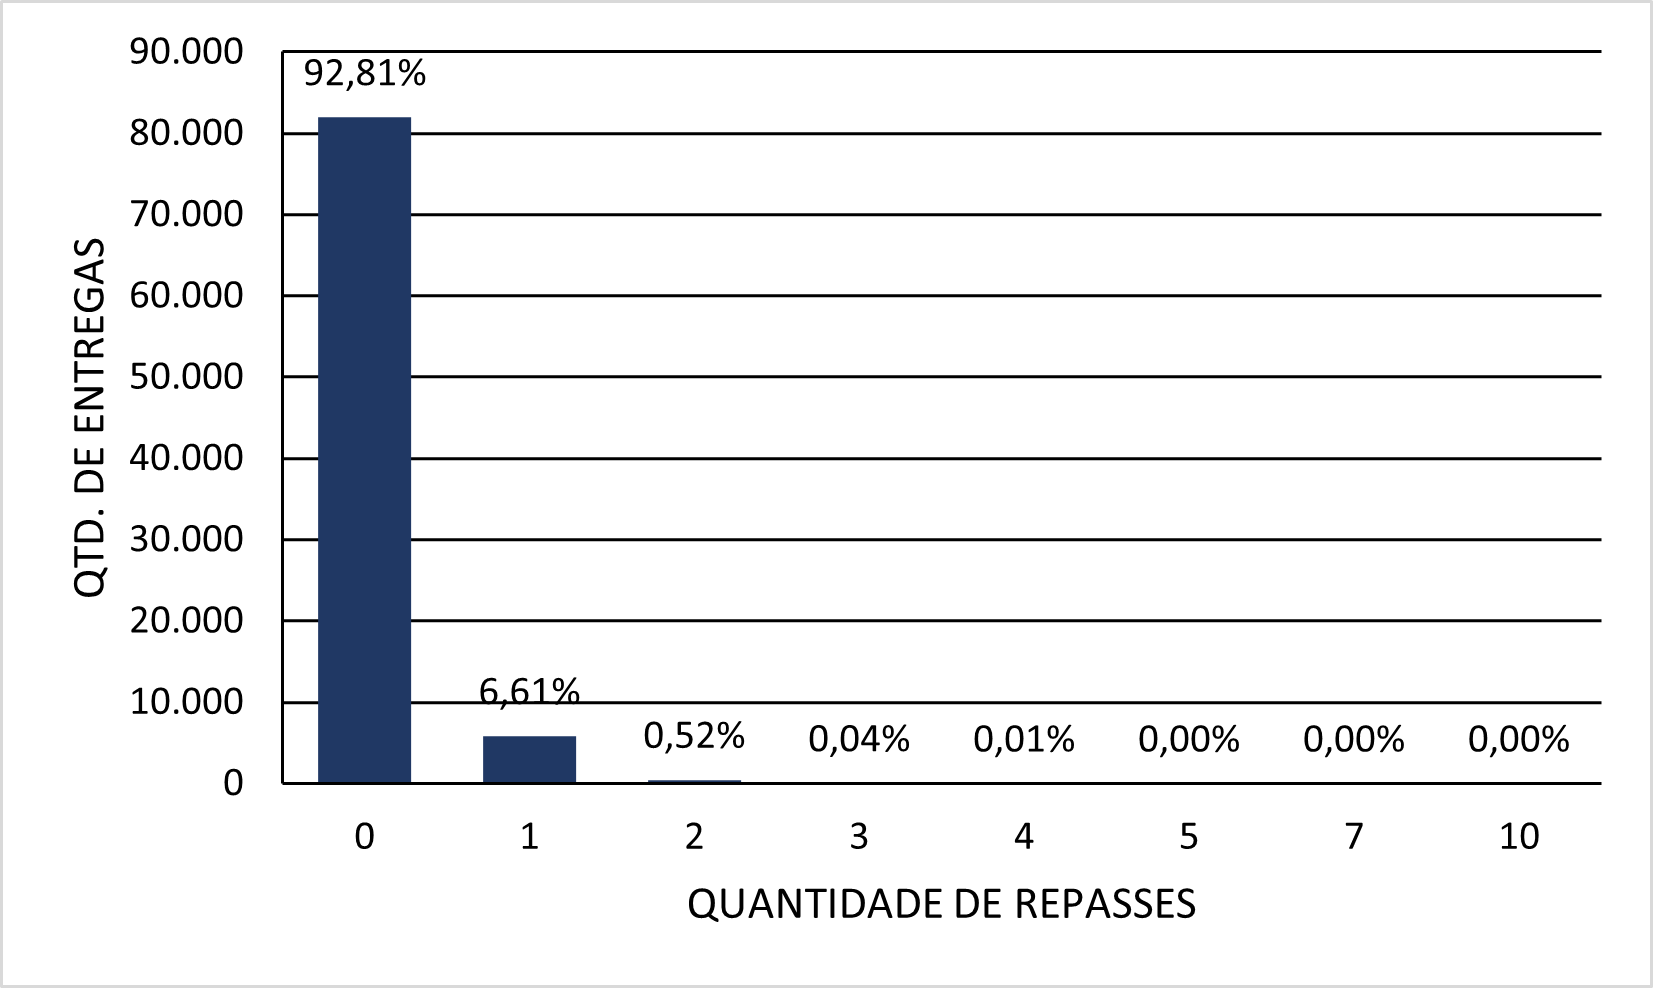
\includegraphics[width=0.5\textwidth]{images/5_emp_bebidas/excel_based/qtde_repasses1.png}
    \caption*{\ Fonte: Produzido pelos autores Fernandes \& Alves}
    \label{fig:Repasses}
\end{figure}

Em adição ao histograma da Figura \ref{fig:Repasses}, é possível observar as ocorrências de repasses nas rotas como um todo a partir da Figura \ref{fig:RepassesRotasBebidas}.
Nela, verifica-se, como supramencionado, que 52\% das rotas apresentam ao menos 1 repasse, sendo que a quantidade máxima de repasses ocorridos em uma única rota no intervalo estudado foi de 20 repasses.
Ademais, identifica-se que 93\% das rotas têm até 4 repasses e 99\% das rotas têm até 9 repasses.

\begin{figure}[H]
    \centering
    \caption{Histograma da quantidade de repasses sofrido por cada cada rota.}
    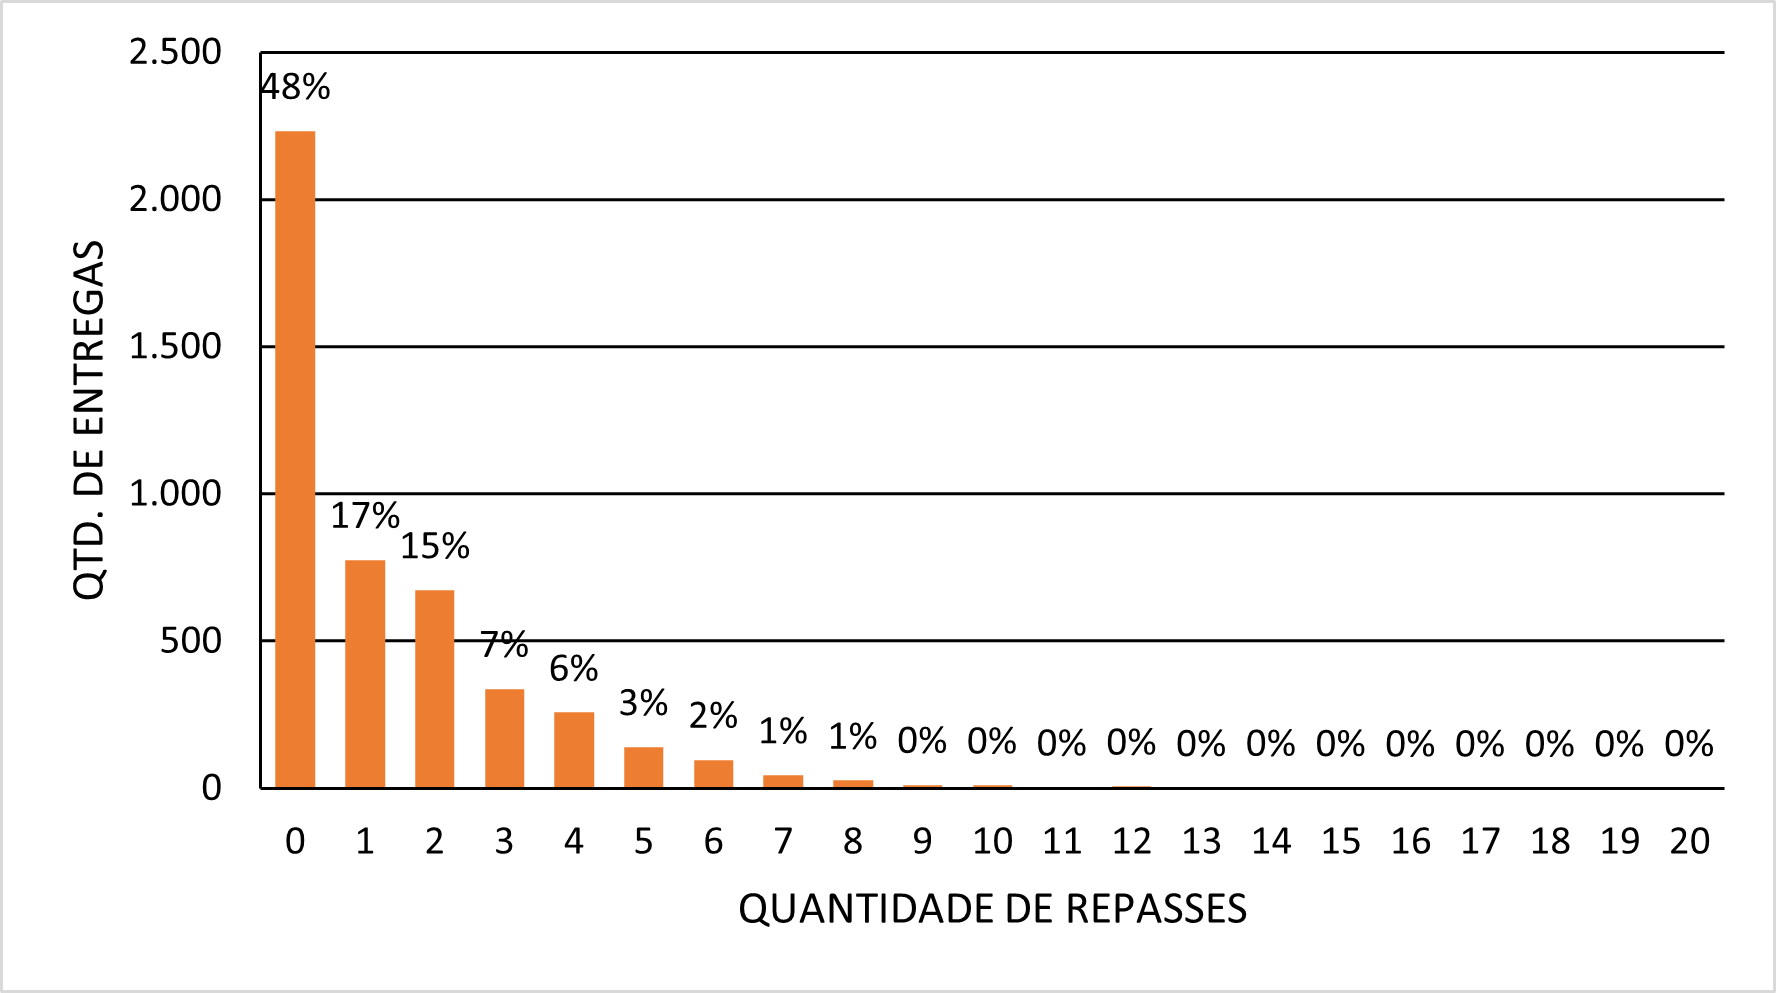
\includegraphics[width=0.5\textwidth]{images/5_emp_bebidas/excel_based/qtde_repasses2.png}
    \caption*{\ Fonte: Produzido pelos autores Fernandes \& Alves}
    \label{fig:RepassesRotasBebidas}
\end{figure}

Em sequência, as devoluções representam 2,1\% do volume total de entregas na amostra de dados explorada na presente pesquisa. 
Tais devoluções ocorreram em 3,2\% das entregas discretizadas.

Finalmente, com intuito de simplificar o entendimento do presente tópico, estabelece-se a Tabela \ref{tab:Variaveis_Problema}, onde é possível observar as principais características citadas de cada medida principal do problema. O restante do trabalho discorrerá, essencialmente, sobre estas três variáveis e quanto à sua relação com outros aspectos intrínsecos à operação ou à configuração da malha viária.

\singlespacing
\begin{table}[htb]
    \centering
    \caption{Resumo das variáveis do problema identificados preliminarmente.}
    \begin{tabular}{|c|c|c|}
    \rowcolor[HTML]{BFBFBF} 
    \hline
    \textbf{Variável} & \textbf{Descrição} & \textbf{Ocorrência} \\ \hline
    Repasse & \begin{tabular}[c]{@{}c@{}}Entregas não realizadas em primeira tentativa.\end{tabular} & 7,2\% \\
    Devolução & \begin{tabular}[c]{@{}c@{}}Volume não entregue e devolvido para o CD.\end{tabular} & 2,1\% \\
    NAS & \begin{tabular}[c]{@{}c@{}}Entrega realizada em sequência diferente da planejada.\end{tabular} & 91,4\% \\ \hline
    \end{tabular}%}
    \caption*{Fonte: Produzido pelos autores Fernandes \& Alves}
    \label{tab:Variaveis_Problema}
\end{table}
\onehalfspacing

Por fim, cita-se que na amostragem do estudo de caso da empresa de bebidas, 91,4\% das entregas feitas tiveram uma alteração em suas ordens sequenciais, valor bastante expressivo e que significa dizer, com efeito, que apenas 8\% das entregas ocorreram de acordo com a ordem ou sequência planejada. Apesar de ser a variável mais frequente apresentada, ela tem um menor impacto direto na perspectiva macroscópica da empresa quando comparada com a devolução, por exemplo, a qual implica no não faturamento de produtos e, portanto, gera maior preocupação para o cotidiano da empresa. 

%%%%%%%%%%%%%%%%%%%%%%%%%%%%%%%%%%%%%%%%%%%%%%%%%%
\section{Impactos econômicos, ambientais e legais} \label{sec:impactoBebidas}

Como detalhado na Seção \ref{RelevanciaTema}, a problemática estudada no presente trabalho acarreta em efeitos negativos de caráter econômico, social e ambiental. Assim, no âmbito do estudo de caso da empresa de bebidas brasileira, é possível definir dois parâmetros primordiais a partir da base de dados fornecida para entender e quantificar tais impactos: distância adicional percorrida e tempo extraordinário de entrega.

A distância adicional percorrida em um roteiro de entregas é caracterizada pela distância que o veículo percorre além do que estava previsto inicialmente para realização de todas as entregas. 
Conforme apresentado por \citeonline{FLAVIOetal}, o processo de roteirização no estudo de caso em questão - que trata da mesma base de dados da empresa de bebidas - apresentou tendência de se superestimar a distância a ser percorrida pelo veículo de entrega, resultando em erros de programação de distância na casa de 30\%, em média.
De fato, a Figura \ref{fig:DistPlan_vs_distReal} ilustra a distribuição de distâncias reais percorridas em comparação com a distância programada, totalizando mais de 15.000 km percorridos adicionalmente.
Esta distância excedente pode resultar em um acréscimo de custos operacionais para a empresa em questão, devido ao maior consumo de combustíveis, maior custo de manutenção associado à utilização dos veículos e também ao maior custo da cadeia de recursos humanos (motorista, auxiliares, entre outros) que afetam a sustentabilidade do sistema operacional.

\begin{figure}[ht]
    \centering
    \caption{Comparativo entre distância real percorrida e distância planejada de cada rota}
    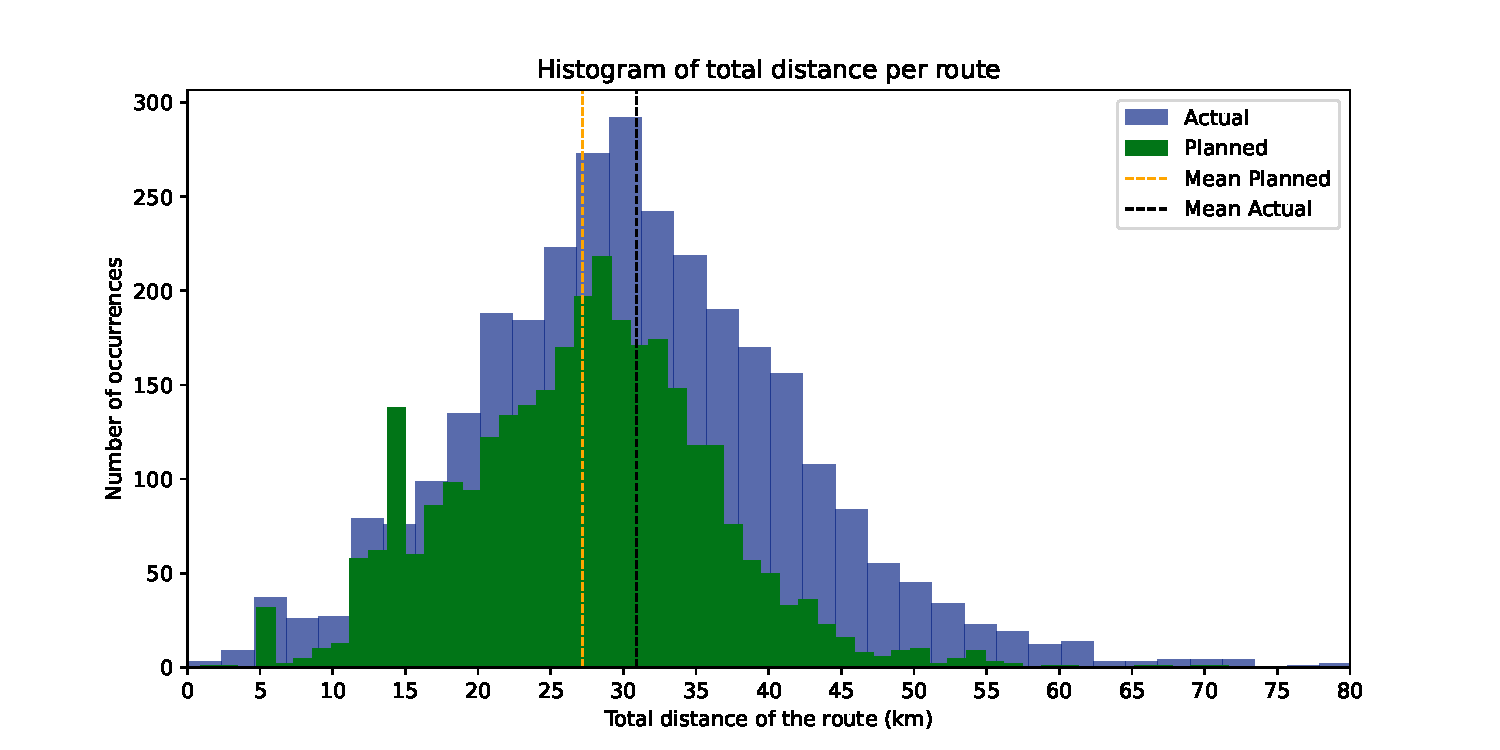
\includegraphics[width=0.8\textwidth]{images/5_emp_bebidas/excel_based/distances_histogram.pdf} 
    \caption*{\ Fonte: Produzido pelos autores Fernandes \& Alves}
    \label{fig:DistPlan_vs_distReal}
\end{figure}

Por outro lado, a distância adicional percorrida impacta, também, ambientalmente devido à emissão de gases contribuintes ao efeito estufa.
Se for considerado que um veículo típico de entregas urbanas consome cerca de 1 litro de diesel a cada 5,5 quilômetros percorridos, considerando-se o consumo urbano de gasolina de um \textit{Volkswagen Delivery Express 2.8} como referência \citeonline{Ramos2021} e que há uma emissão média de 3,2 kg de \ce{CO2} por litro de diesel consumido (que inclui a produção, a distribuição e a queima do diesel, como estimado por \citeonline{Carvalho2011}, a quilometragem percorrida extraordinariamente durante os seis meses de operação analisados passa a representar um total de cerca 7,9 toneladas (t) \ce{CO2} emitidos.
Ou seja, em média são gerados em torno de 16 toneladas adicionais de \ce{CO2} por ano somente no CD estudado.

Finalmente, a Figura \ref{fig:DistPlan_vs_distReal_CORRELACAO} apresenta a correlação entre distância real percorrida e distância planejada levantada pelos autores, obtendo-se a relação de cerca de 10\%, valor abaixo do evidenciado por \citeonline{FLAVIOetal} porém ainda assim representativo para as análises do presente trabalho.

\begin{figure}[ht]
    \centering
    \caption{Distância real percorrida em função da distância planejada}
    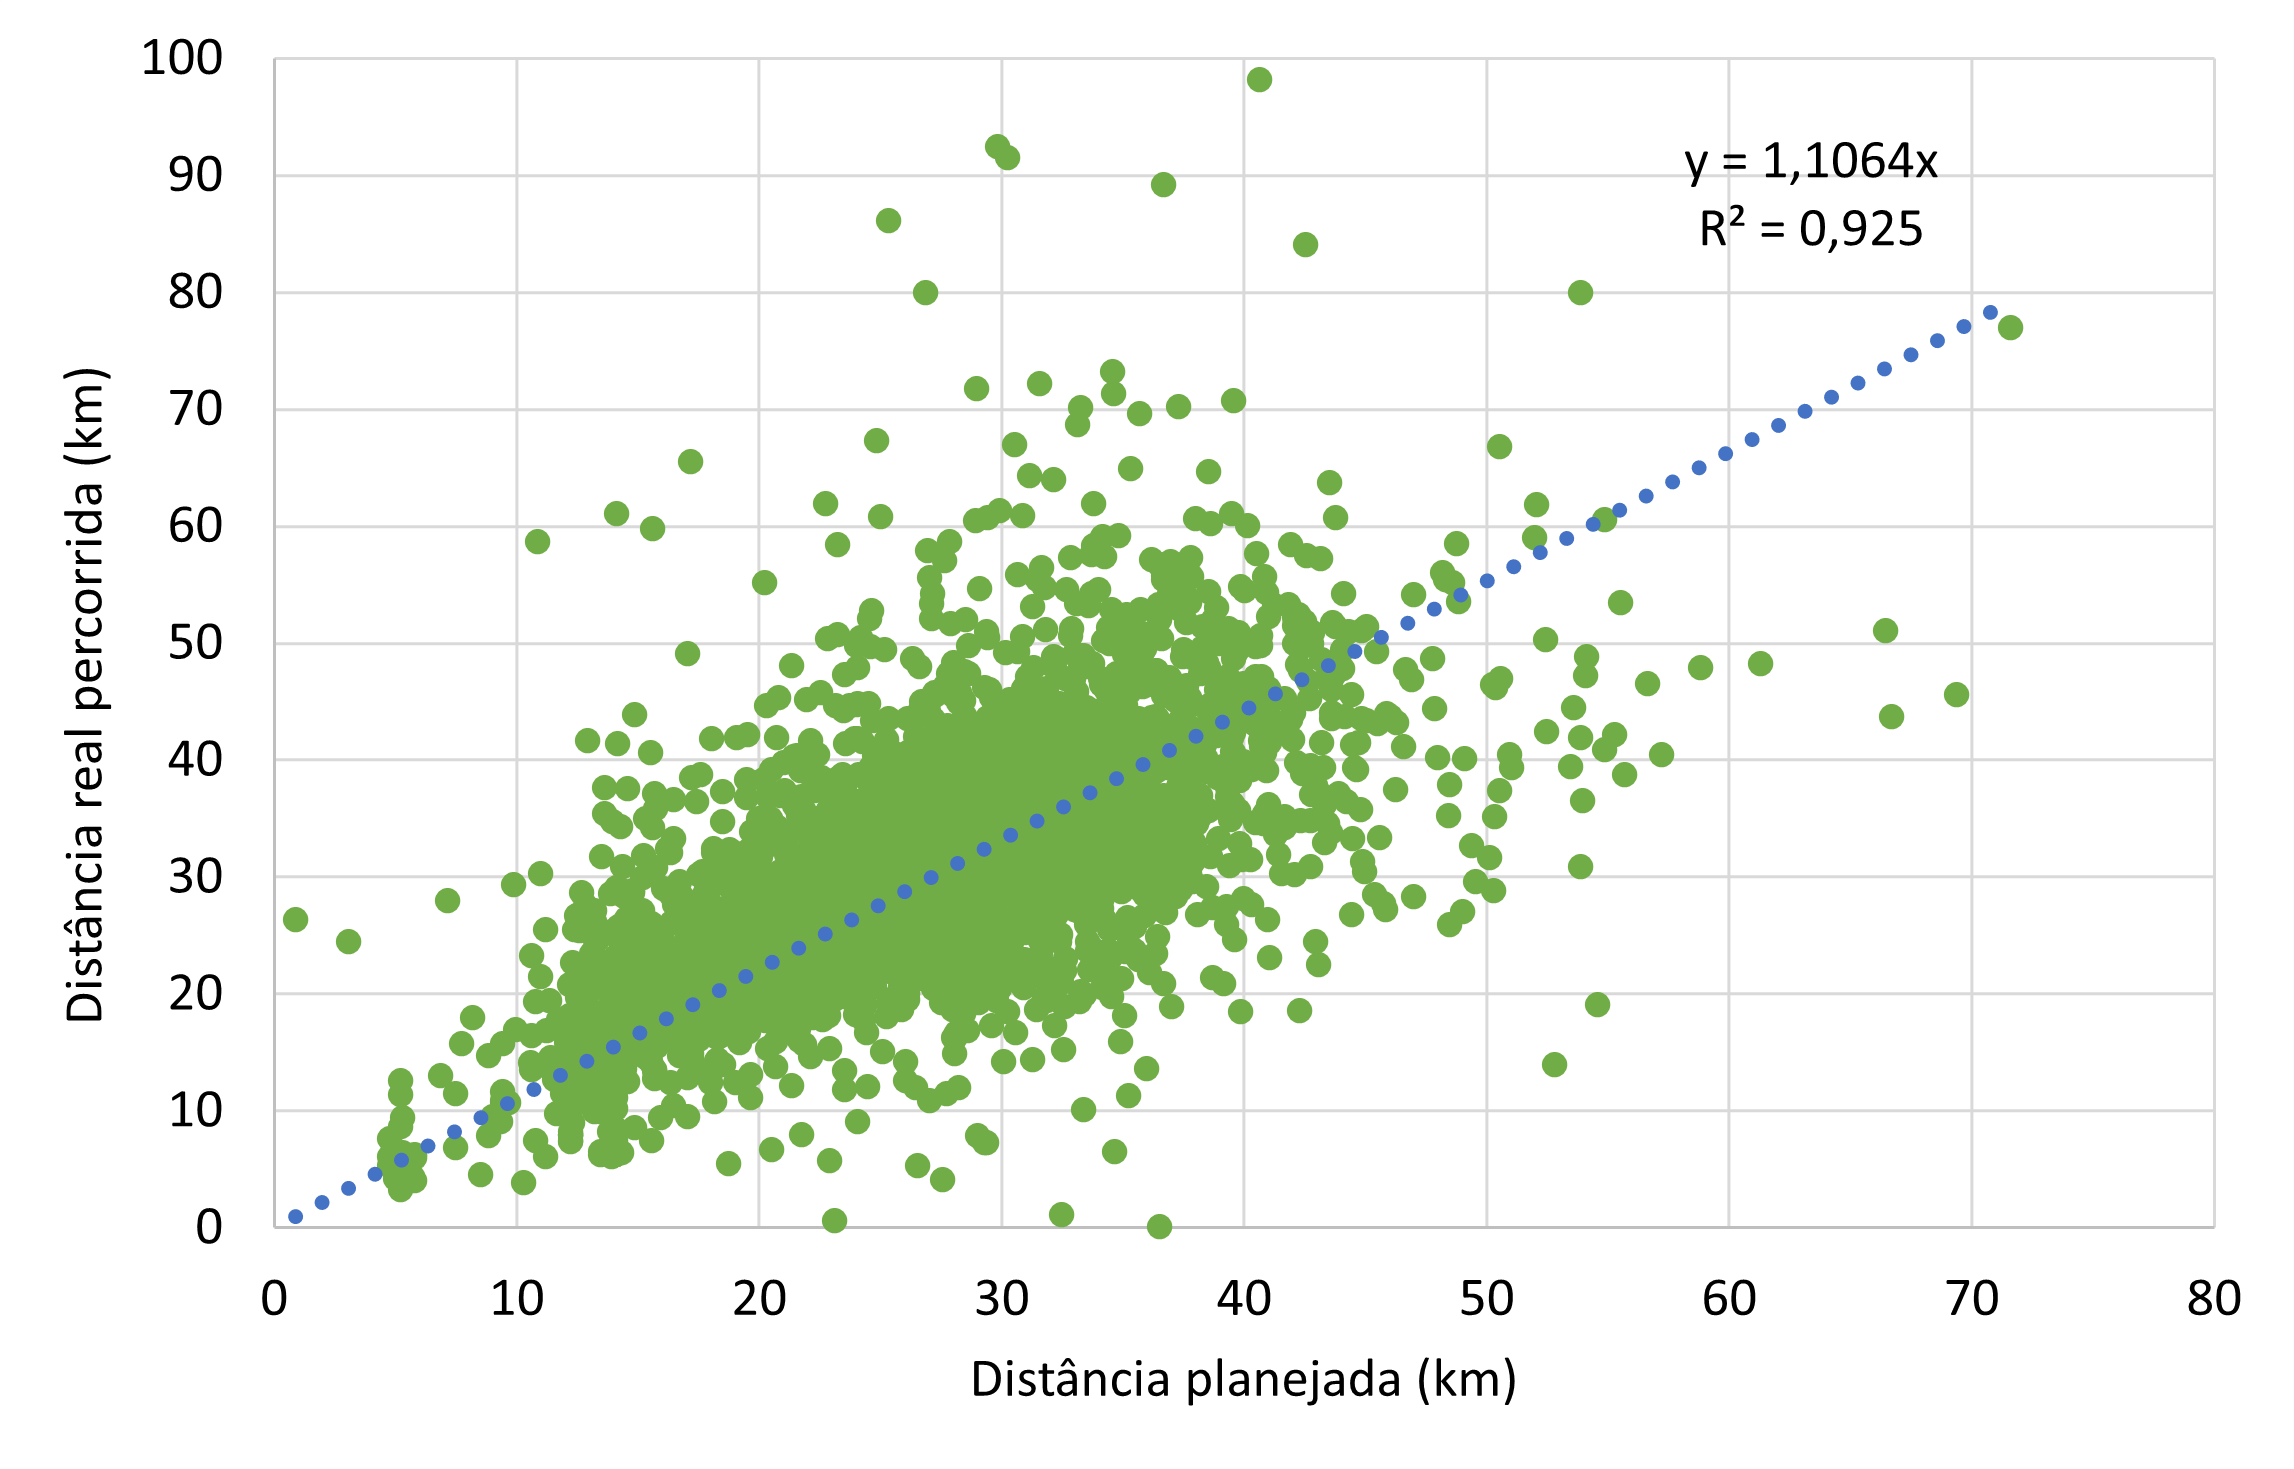
\includegraphics[width=0.6\textwidth]{images/5_emp_bebidas/excel_based/dist_plan_vs_real.png} 
    \caption*{\ Fonte: Produzido pelos autores Fernandes \& Alves}
    \label{fig:DistPlan_vs_distReal_CORRELACAO}
\end{figure}

Outro parâmetro que pode ser analisado a fim de se caracterizar o impacto de não aderência é o tempo extraordinário de entrega, que por sua vez poderá implicar em problemas legais à empresa devido questões trabalhistas. Como apresentado por \citeonline{FLAVIOetal}, para cada conjunto de entregas por veículo há uma forte preocupação em manter a jornada líquida abaixo de 10h20, que é o limite permitido de acordo com a legislação trabalhista. Sendo assim, uma vez que atrasos relacionados à não aderência pode afetar o descumprimento da limitação de jornada de trabalho, há uma preocupação institucional de que o tempo excedente seja controlado e mitigado o máximo possível.

Estes fatores configuram as duas principais fontes de preocupação que justificam o estudo sobre a aderência ao planejamento de entregas no estudo de caso em questão. 

%%%%%%%%%%%%%%%%%%%%%%%%%%%%%%%%%%%%%%%%%%%%%%%%%%%%%%%%%%%%%%%
\section{Visita Técnica}  \label{sec:visita_tecnica}

No dia 17 de junho de 2022 os autores realizaram uma visita técnica ao CD da empresa de bebidas concedente dos dados analisados.
%
É importante destacar que o CD visitado não é o mesmo centro estudado por meio da base de dados, porém para o escopo da pesquisa a diferença entre os dois CDs (visitado e estudado) é considerada desprezível.
%
Ademais, convém ressaltar que há uma lacuna temporal entre os valores observados na base de dados e a realidade observada na prática, visto que a visita ocorreu cerca de sete anos após a coleta de informações para a base de dados estudada.
%
Em sete anos de operação alguns contextos podem se alterar, como é o caso da capacidade, oferta e demanda da empresa, representada pelas variação das quantidades de clientes, SKUs e frota disponível ao longo dos anos.
%
Portanto foi dado foco nos procedimentos que não tenham sido alterados significativamente entre o período de registro dos dados e o momento da visita.
%

De início, uma primeira informação que se destacou para os autores durante a visita foi a diferenciação dos veículos de entrega de acordo com a sua capacidade.
Embora acreditava-se que os veículos eram todos de um mesmo modelo, o que se verificou por meio da visita foi que a empresa opera com pelo menos 3 tipos diferentes de caminhões por dia, sendo eles: caminhão 6 baias, caminhão 10 baias e caminhão \textit{bi-truck}.
Os caminhões modelo \textit{bi-truck} são de maior capacidade, e portanto atendem somente clientes que exigem volumes de entrega mais elevados, como é o caso de supermercados e outros clientes de segmento \textit{off-trade}, i.e. que em geral funcionam como ponto de revenda para o consumidor e não como estabelecimento de consumo. 
As entregas do \textit{on-trade} por sua vez são realizadas pelos caminhões de 6 ou de 10 baias, a depender do volume de entregas. 
É importante destacar que durante o trabalho foram estudadas apenas entregas relativas ao segmento de \textit{off-trade}, visto que é neste setor que o número de entregas por veículo é de fato expressivo.
A decisão sobre qual tipo de veículo utilizar para cada rota é tomada pelo software de roteirização da empresa, que será descrito mais abaixo.

Outro aspecto importante descoberto durante a visita foi a relação entre os tipos de veículo e a largura das vias.
Por se tratar especialmente de uma região metropolitana e até mesmo periférica da cidade de São Paulo, alguns dos clientes estão posicionados em ruas paralelas de menor largura, o que em alguns casos impede a utilização de veículos de capacidade mais elevada, que é o caso dos caminhões de 10 baias.
Desta forma, durante a etapa de planejamento o time de especialistas necessita verificar a compatibilidade entre PDEs e capacidade do caminhão, podendo realizar alguns ajustes que estejam mais visíveis.
Contudo nem sempre é possível determinar as rotas ideais uma vez que informações de largura de via não são de fácil acesso aos usuários comuns, tampouco para os especialistas de planejamento.
O que se faz para contornar essa situação, em geral, é padronizar a equipe de entregas por região e veículo, de modo que um mesmo motorista tenda a percorrer percursos similares e dessa forma já consiga prever de antemão quais os empecilhos que podem se apresentar durante a rota.

Adicionalmente identificou-se uma possível segmentação de clientes durante a visita. 
Foi mencionado que alguns clientes recebiam prioridade de entrega por participarem de algum programa de clientes \textit{``VIPs''}, o que poderia significar em piores valores de NAS devido a uma estratégia customizada da empresa. 
Tal aspecto evidencia uma limitação da base de dados descrita na seção \ref{sec:realidade_empresa}, uma vez que não houve qualquer diferenciação entre os tipos de clientes.

Já quanto à programação das rotas em si, esta é realizada diariamente através de \textit{software} solução de mercado obtido pela empresa e utilizada em escala nacional pelos seus diferentes CDs.
Diariamente a equipe de planejamento precisa atualizar no sistema da empresa qual é a disponibilidade real de frota para realização de entregas do dia seguinte, este cadastro ocorre por volta das 17 horas, ou seja, quase no final do expediente.
Uma vez cadastrados os dados no sistema, a roteirização será feita em segundo plano utilizando como base os pedidos que foram confirmados pelos clientes até o fim do dia.
O processo não leva mais de duas horas para ser concluído, porém ao se obter o resultado da roteirização muitas vezes são realizados diversos ajustes manuais de modo a compatibilizar o resultado extraído do simulador com a realidade experienciada pelos planejadores e operação.

Durante o expediente de operação, que geralmente vai de 8 da manhã até 7 da noite em dias convencionais, a equipe de planejamento de rotas fica disposta no CD da empresa em local dedicado exclusivamente para acompanhamento das entregas e replanejamento de tentativas mal-sucedidas. 
Sempre que uma entrega não pôde ser realizada, a equipe de planejamento é acionada para verificar qual o melhor horário para a operação retornar ao PDE naquele dia, além de registrar os motivos da não realização das entregas.
Um painel em formato de \textit{dashboard} é utilizado para acompanhamento das rotas de entrega ao longo do expediente, conforme evidenciado na Figura \ref{fig:painel_repasses}, em que cada linha representa uma rota diferente e cada círculo representa um diferente PDE.
A cor verde indica que a entrega naquele PDE foi concluída com sucesso, a vermelha significa que não foi possível entregar e que está confirmado que haverá devolução, enquanto que a cor roxa indica que já foi feita tentativa sem sucesso porém a entrega foi remarcada para outro horário (ou seja, ocorrência de repasse).

\begin{figure}[htb]
    \centering
    \caption{Painel de acompanhamento das rotas de entregas registrado no dia da visita}
    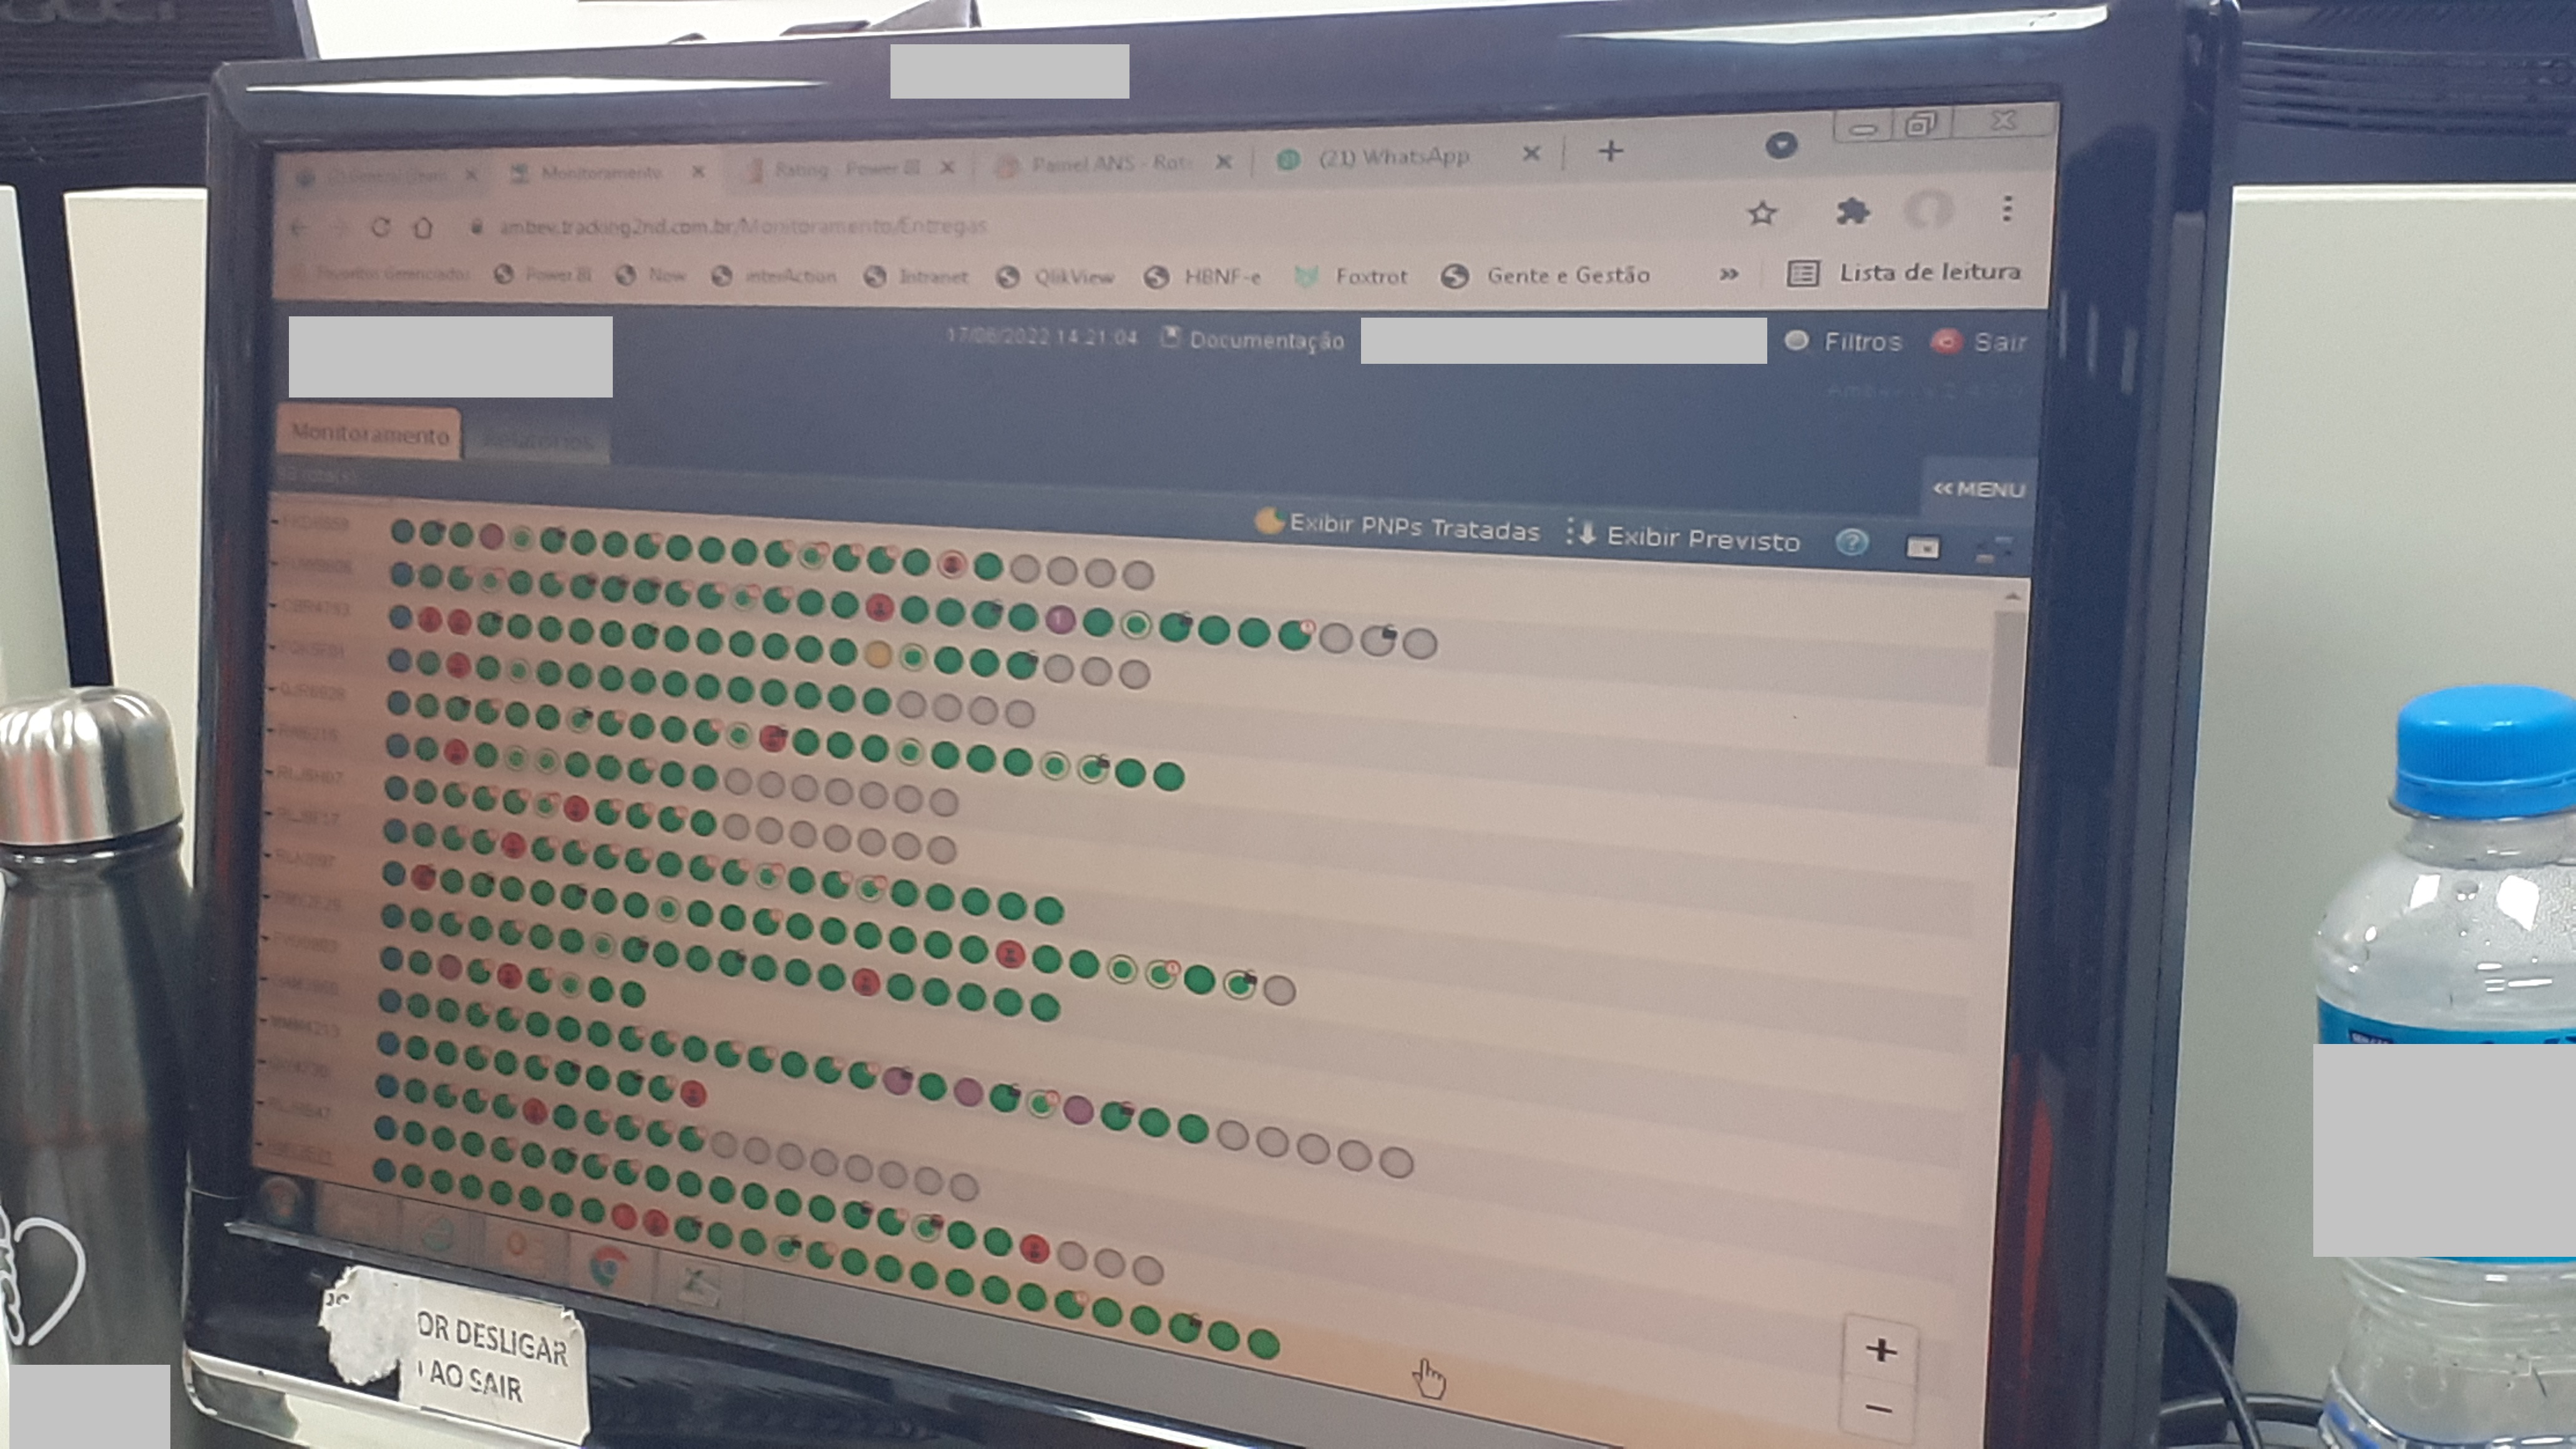
\includegraphics[width=0.8\textwidth]{images/5_emp_bebidas/painel_rotas_CDD_diadema.jpg}
    \caption*{Fonte: Produzido pelos autores Fernandes \& Alves}
    \label{fig:painel_repasses}
\end{figure}

Ademais, através contato direto com a equipe operacional, foi possível estabelecer novas linhas de análise, antes não consideradas. Uma tese levantada conjuntamente, foi de que o calendário (dia da semana, época do mês, feriados, etc.) pode ter influência direta nos problemas estudados. 
%
Outra informação relevante que pôde ser estabelecida na visitação técnica foi acerca do quão rigorosa a equipe operacional é com devoluções. Eles estabelecem um critério de bloqueio dos PDE que apresentam reincidência de devoluções, ou seja, que realizam devoluções repetidamente. Essa informação, futuramente, pode ser considerada na possibilidade de se observar, na base de dados, qual o comportamento, ao longo do tempo, para com os PDEs com maiores índices de devoluções.

A visita técnica em questão possibilitou a adição de conceitos e visões externas ao trabalho, de modo que os autores puderam validar algumas das hipóteses e, principalmente, entender na prática como funcionam algumas das rotinas de distribuição de entregas de última milha na região estudada.


%%%%%%%%%%%%%%%%%%%%%%%%%%%%%%%%%%%%%%%%%%%%%%%%%%%%%%%%%%%%%%%
\section{Perfil das rotas} \label{sec:analise_base_dados}

Ao inspecionar a base de dados disponibilizado para o estudo, elencou-se cinco parâmetros que poderiam apresentar alguma correlação com os problemas estudados, são eles: Posição sequencial do PDE dentro de sua rota; Frequência média de entregas do PDE; Veículo utilizado para realizar a entrega; Horário em que a entrega foi realizada; e Volume de caixas da entrega.
Estes valores bem como a relação com o problema atual estão descritos nos itens a seguir.

\subsection{Posição Sequencial}

Como apresentado na seção \ref{sec:realidade_empresa}, a base de dados inclui informação sobre qual posição cada PDE ocupou na sequência de entregas de cada rota.
É possível induzir que a posição que o PDE ocupou na sequência de entregas pode ser relevante para explicar alguns dos fenômenos analisados.
Isso se dá pela tese de que os motoristas podem ter problemas mais frequentemente com alguma posição específica da sequência, especialmente as mais extremas – primeiras ou últimas.

Desta forma, identificou-se que, a NAS tem uma relação proporcional com a variável ``posição sequencial'', enquanto os repasses apresentam uma relação inversamente proporcional, como observa-se nas Figuras \ref{fig:PosicaoSequencial} e \ref{fig:PosicaoSequencialRS}.

\begin{figure}[H]
    \caption{Correlação entre fenômeno estudado e a posição sequencial do PDE na rota.}
    \begin{subfigure}{.64\textwidth}
        \centering
        % include first image 
        \caption{Relação Gráfica entre as variáveis e a Posição Sequencial.}
        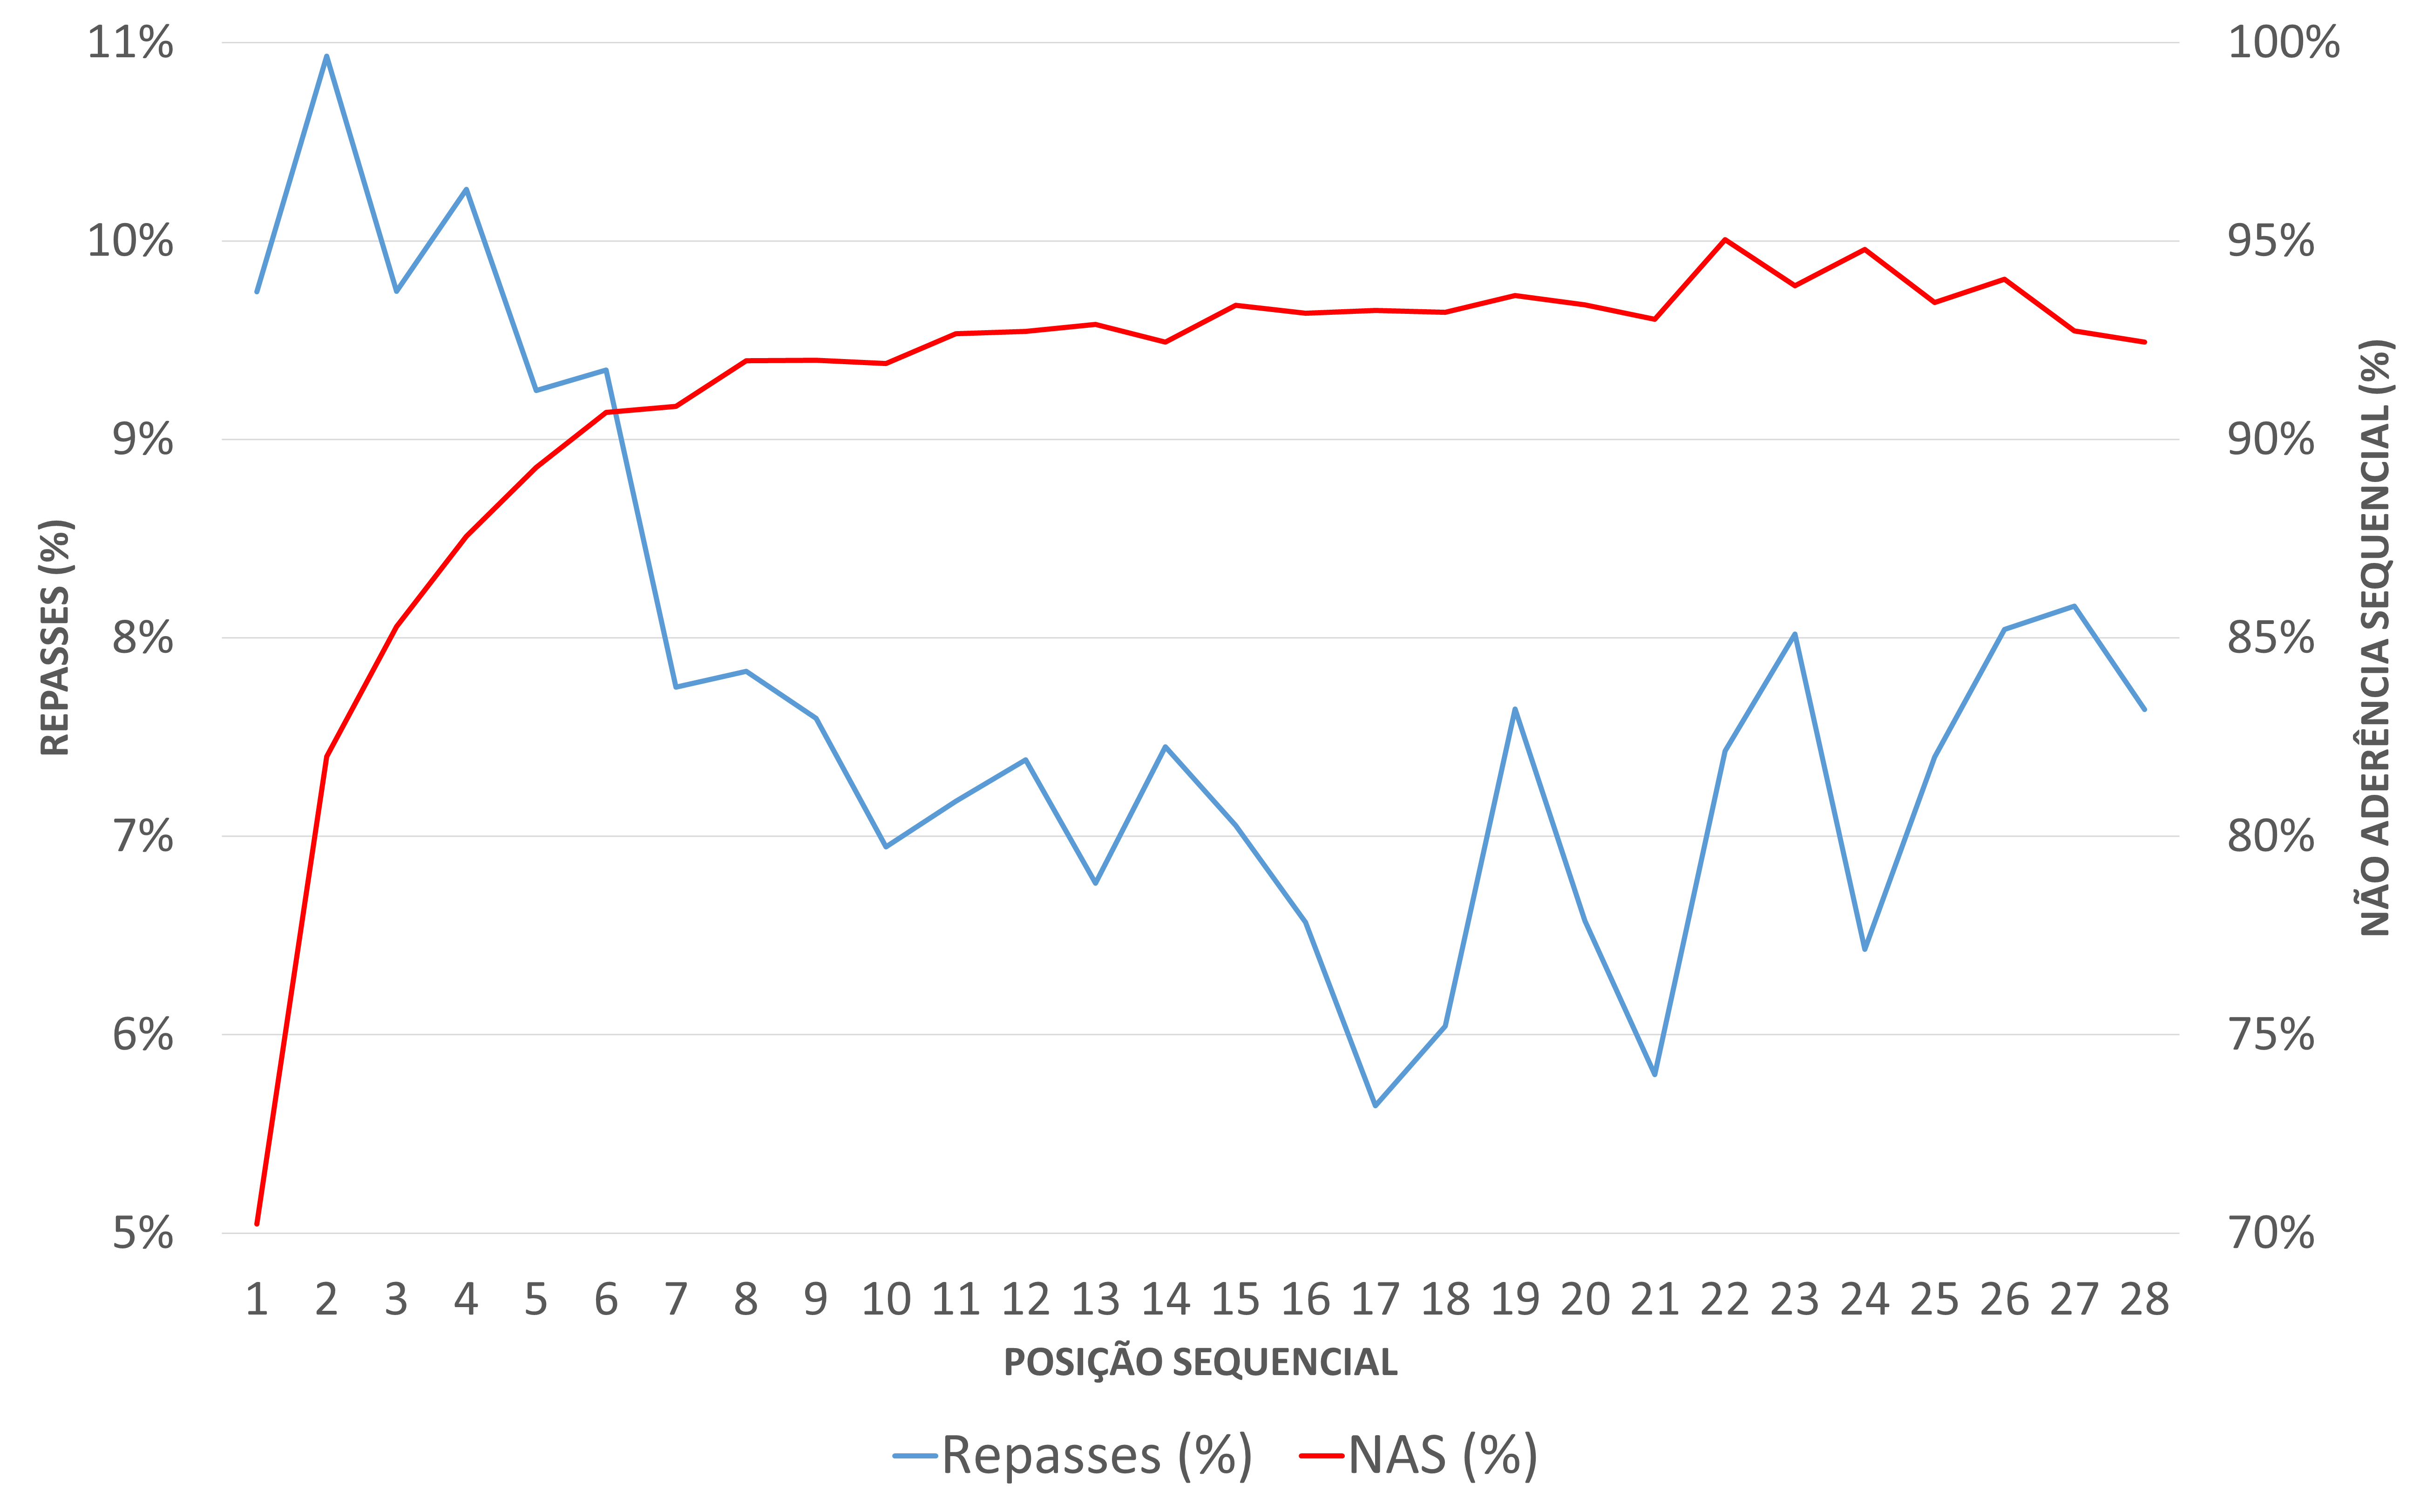
\includegraphics[width=.98\linewidth]{images/5_emp_bebidas/excel_based/PosicaoSequencial.png}
        \label{fig:PosicaoSequencial}
    \end{subfigure}
    \begin{subfigure}{.35\textwidth}
      \centering
      % include second image
      \caption{Estatísticas da Regressão Linear.}
      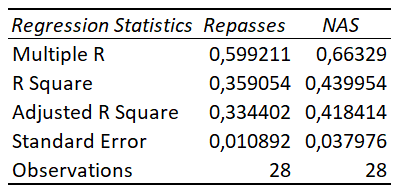
\includegraphics[width=.88\linewidth]{images/5_emp_bebidas/excel_based/PosicaoSequencial_RS.png}
      \label{fig:PosicaoSequencialRS}
    \end{subfigure}
    \caption*{\ Fonte: Produzido pelos autores Fernandes \& Alves}
\end{figure} % Posicao Sequencial

É importante destacar que a relação observada, porém, é inversa para cada problema. 
Ou seja, identifica-se que a ocorrência de repasses é maior nas primeiras posições, enquanto a aderência sequencial é menor nas últimas posições.
Assim, observa-se que cada problema, mesmo tendo um comportamento único, pode ser explicado através da mesma variável.

\subsection{Frequência}

A partir da base de dados fornecida, outra informação que é possível construir é a frequência média de entregas que cada PDE recebe. 
Isso pode ser obtido a partir da informação da data em que foi realizada cada entrega. 
Tal informação, empiricamente, pode ser estabelecida como uma potencial variável relacionada aos problemas estudados, assumindo-se que o motorista do veículo de entregas pode ser influenciado positivamente pelo nível de conhecimento que ele tem do PDE – seus receptores, o espaço de descarga, as vias de acesso, etc. 
Por outro lado, estabelece-se a possibilidade de que a alta frequência de entregas em determinado PDE impacte negativamente na aderência ao sequenciamento e/ou nos repasses devido a um vínculo de confiança que pode se estabelecer entre os dois agentes citados e, assim, gerar no motorista confiança suficiente para estabelecer sua própria rotina de entregas, ignorando parcial ou totalmente o sequenciamento gerado pelo roteirizador.

Assim, nas Figuras \ref{fig:Frequencia1} e \ref{fig:Frequencia2} é possível observar a relação entre o percentual de repasses e NAS com a frequência de entregas, obtendo aderência suficiente num primeiro momento.

 \begin{figure}[H]
     \caption{Correlação entre a frequência de entregas no PDE e as variáveis-problema.}
     \begin{subfigure}{.64\textwidth}
         \centering
         % include first image 
         \caption{Relação Gráfica entre as variáveis e a Frequência.}
         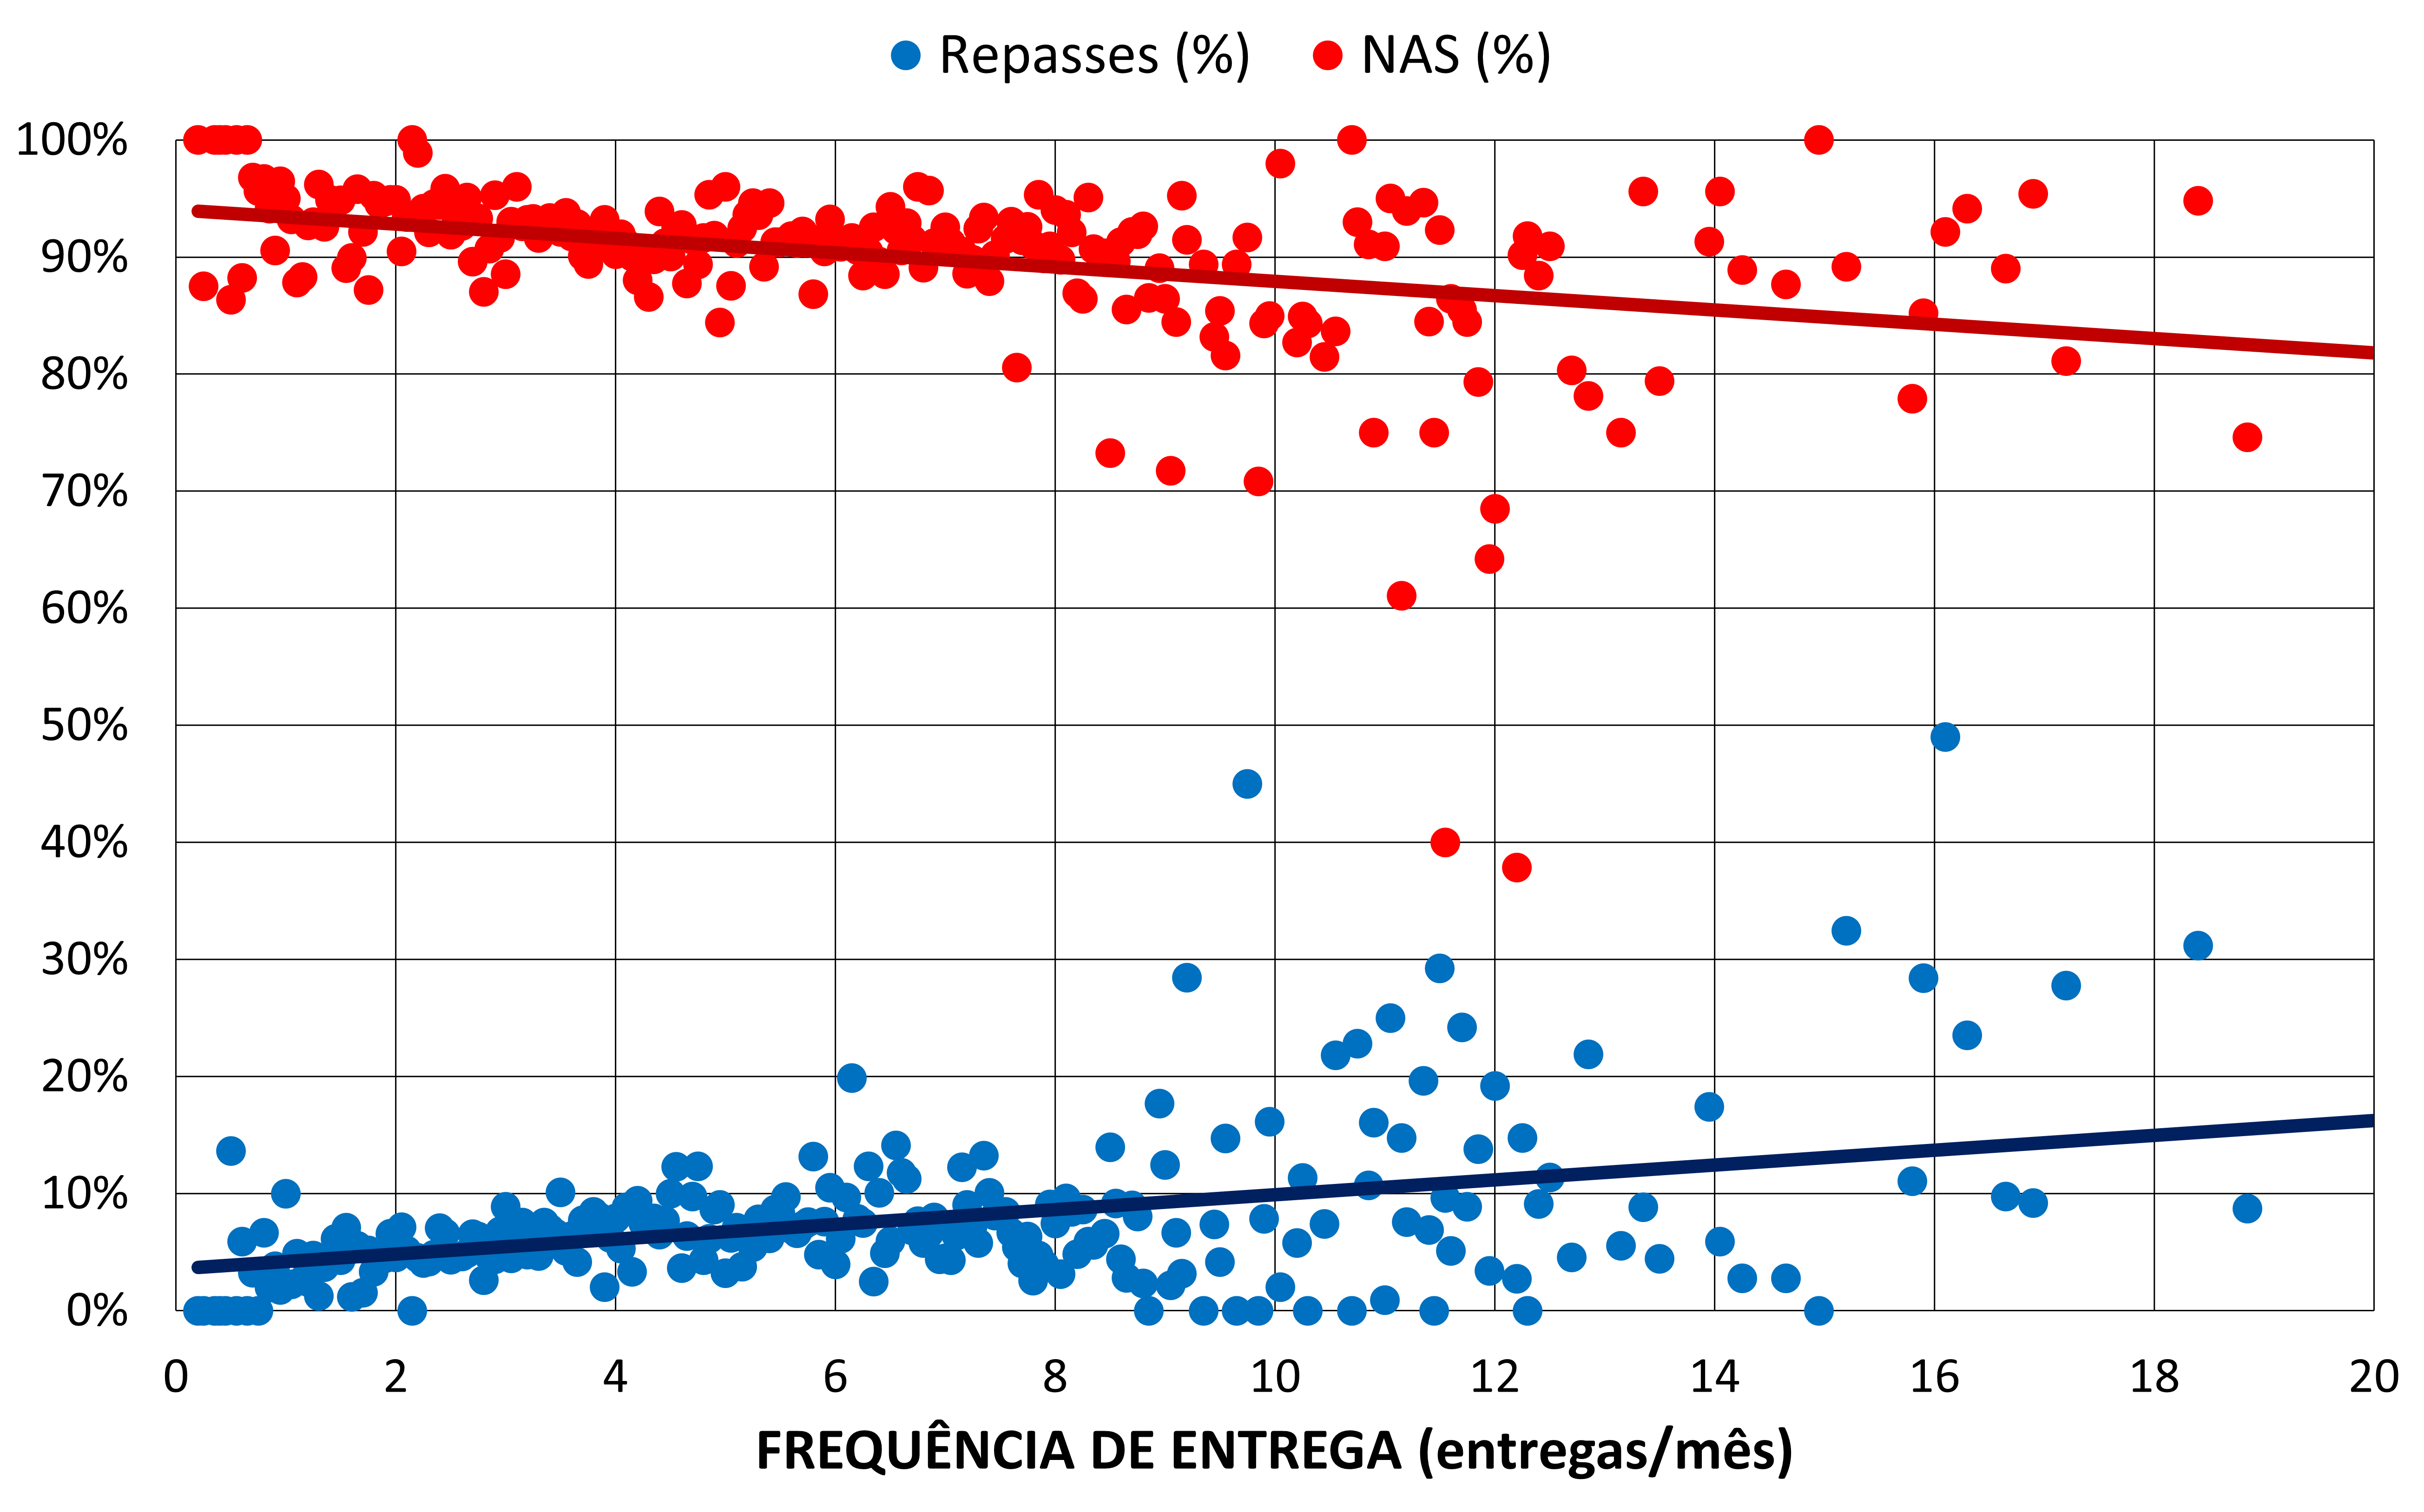
\includegraphics[width=.98\linewidth]{images/5_emp_bebidas/excel_based/Frequencia.png}
         \label{fig:Frequencia1}
     \end{subfigure}
     \begin{subfigure}{.35\textwidth}
       \centering
       % include second image
       \caption{Estatísticas da Regressão.}
       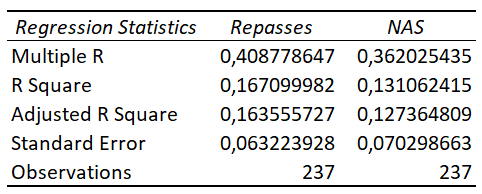
\includegraphics[width=.88\linewidth]{images/5_emp_bebidas/excel_based/Frequencia_RS.png}
       \label{fig:Frequencia2}
     \end{subfigure}
     \caption*{\ Fonte: Produzido pelos autores Fernandes \& Alves}
 \end{figure} % Frequencia

Novamente, observa-se um comportamento inverso no parâmetro como causados dos problemas: enquanto frequências altas (0 $<$ T $<$ 10 dias) indicam maior incidência de repasses, são as frequências baixas (12 dias $<$ T) que apresentam baixa aderência.

Um comentário relevante a se fazer em relação a esta análise é de que a frequência de entregas é uma característica associada ao PDE, reduzindo, assim, a amostragem utilizada para a correlação.
Isso se dá pois, em outras análises, tais como a de posição sequencial, a variável é associada a cada entrega realizada (total de 88.338 entregas), enquanto a frequência é associada ao PDE (total de 4.554 PDEs).

\subsection{Veículo}

Outra análise que pode ser realizada a partir dos dados disponibilizados na base de dados é a contribuição do veículo utilizado para as entregas. 
Na base, é possível identificar qual a placa relativa ao veículo utilizado em cada rota. 
Tal análise pode ser validada a partir da informação obtida através da visitação técnica, como visto na seção \ref{sec:visita_tecnica}, de que o planejamento de entregas busca unificar os veículo à equipe (motorista e ajudante(s)) o mais frequentemente o possível. 
Assim, uma correlação pode insurgir da tese de que cada equipe possui preferências e peculiaridades específicas ao seu comportamento e experiência.

Desta forma, foi investigada a correlação entre a placa veicular e os indicadores de repasse e NAS, como pode ser observado na Figura \ref{fig:Veiculo}, onde é possível identificar a ocorrência de uma possível correlação com ambos os indicadores, demonstrando que algumas equipes podem ter maior tolerância aos repasses e à NAS do que outras.

\begin{figure}[H]
    \centering
    \caption{Comparação entre NAS e repasse para os diferentes veículos utilizados.}
    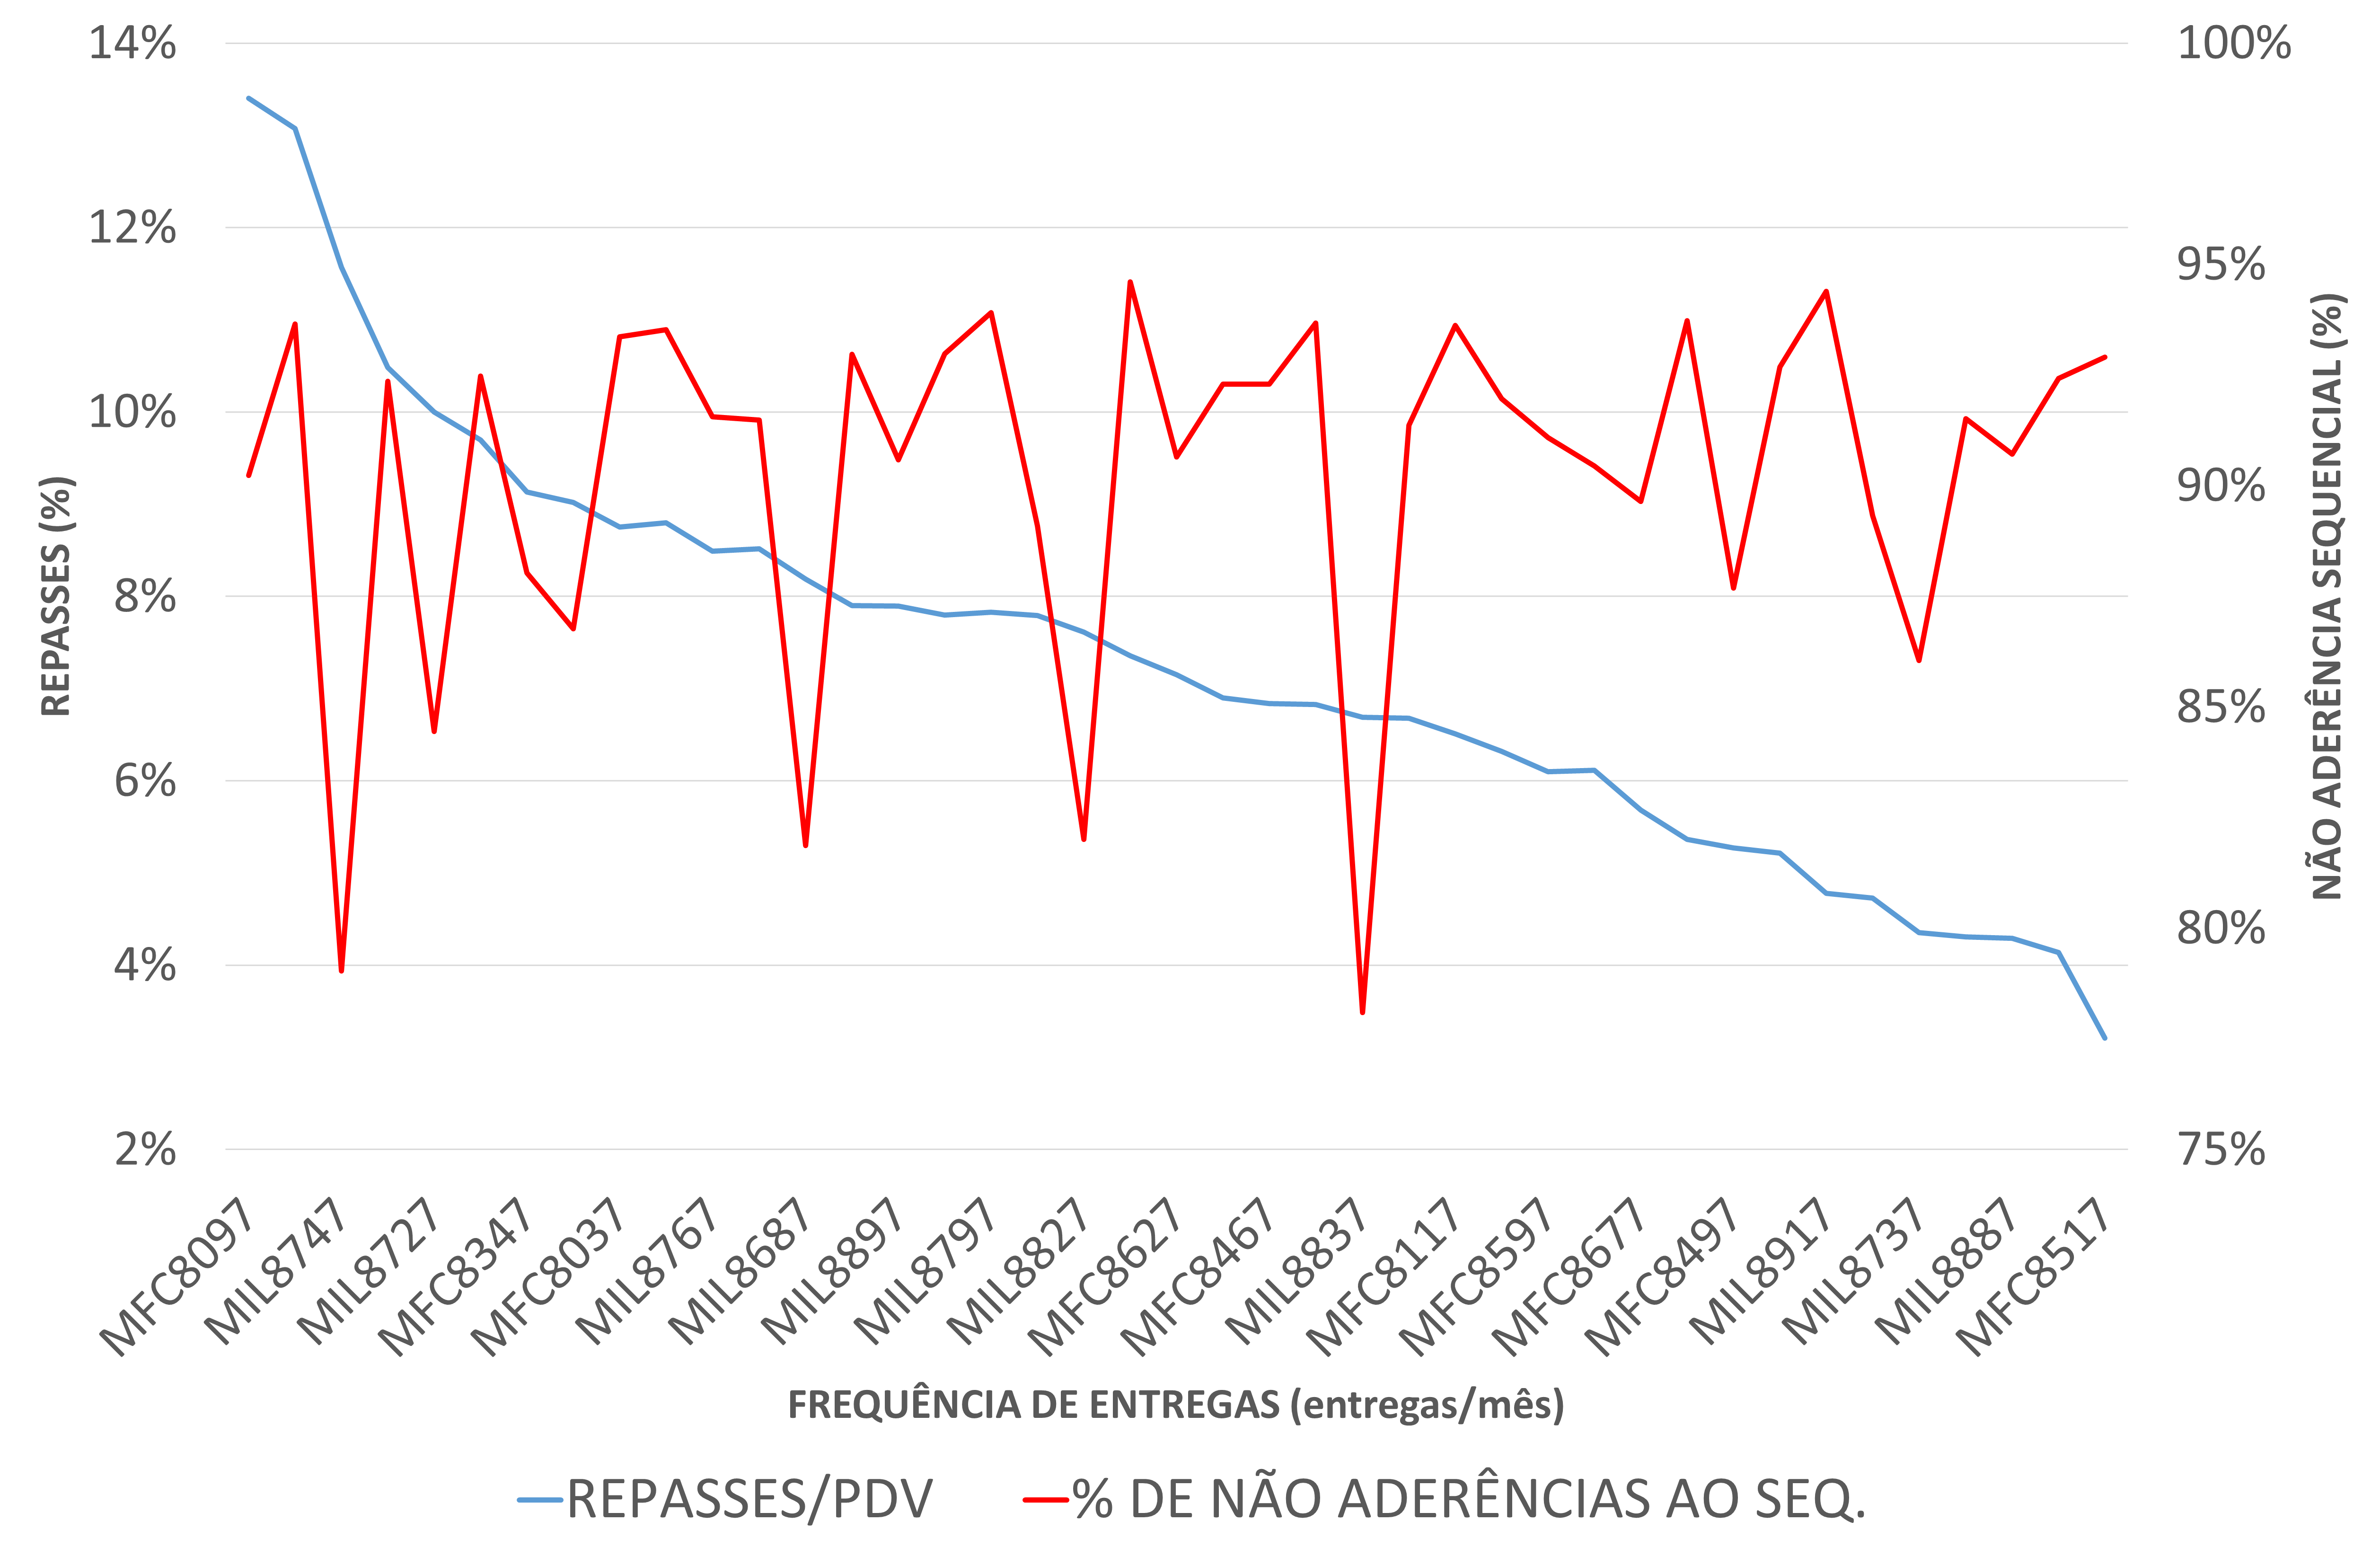
\includegraphics[width=0.8\textwidth]{images/5_emp_bebidas/excel_based/Veiculo.png}
    \caption*{\ Fonte: Produzido pelos autores Fernandes \& Alves}
    \label{fig:Veiculo}
\end{figure} % Veiculo

Um fator relevante a se comentar é a escolha da sequência das placas veicular na Figura \ref{fig:Veiculo}. A escolha foi a favor da ordenação decrescente dos valores de repasse para fins visuais. Naturalmente, o gráfico busca salientar que é possível identificar uma variação considerável das variáveis estudadas, quando organizadas por veículo. Deste modo, confirma-se a tese de que determinadas equipes de entrega podem apresentar maiores tendências de realizar repasses ou NAS do que outras.

\subsection{Horário de Entrega}

Outra análise que pode ser realizada é a de correlação entre as variáveis do problema e o horário no qual a entrega foi realizada.
O horário pode revelar uma correlação com a ocorrência de repasses ou NAS considerando-se o comportamento da equipe de entregas e do cliente receptor. 
Ao longo do dia, diferentes fatores podem ser influenciadores de tais ocorrências, tais como, cansaço dos agentes envolvidos, disponibilidade do receptor, trânsito, entre outros.

As Figuras \ref{fig:Horario} e \ref{fig:HorarioRS} mostram a evolução dos valores médios de repasse (\%) e de NAS (\%) ao longo do dia, considerando a série histórica de cinco meses de entregas.

 \begin{figure}[H]
     \caption{Comparação entre Horário de Entrega e variáveis-problema}
     \begin{subfigure}{.64\textwidth}
         \centering
         % include first image 
         \caption{Relação Gráfica entre as variáveis e o Horário.}
         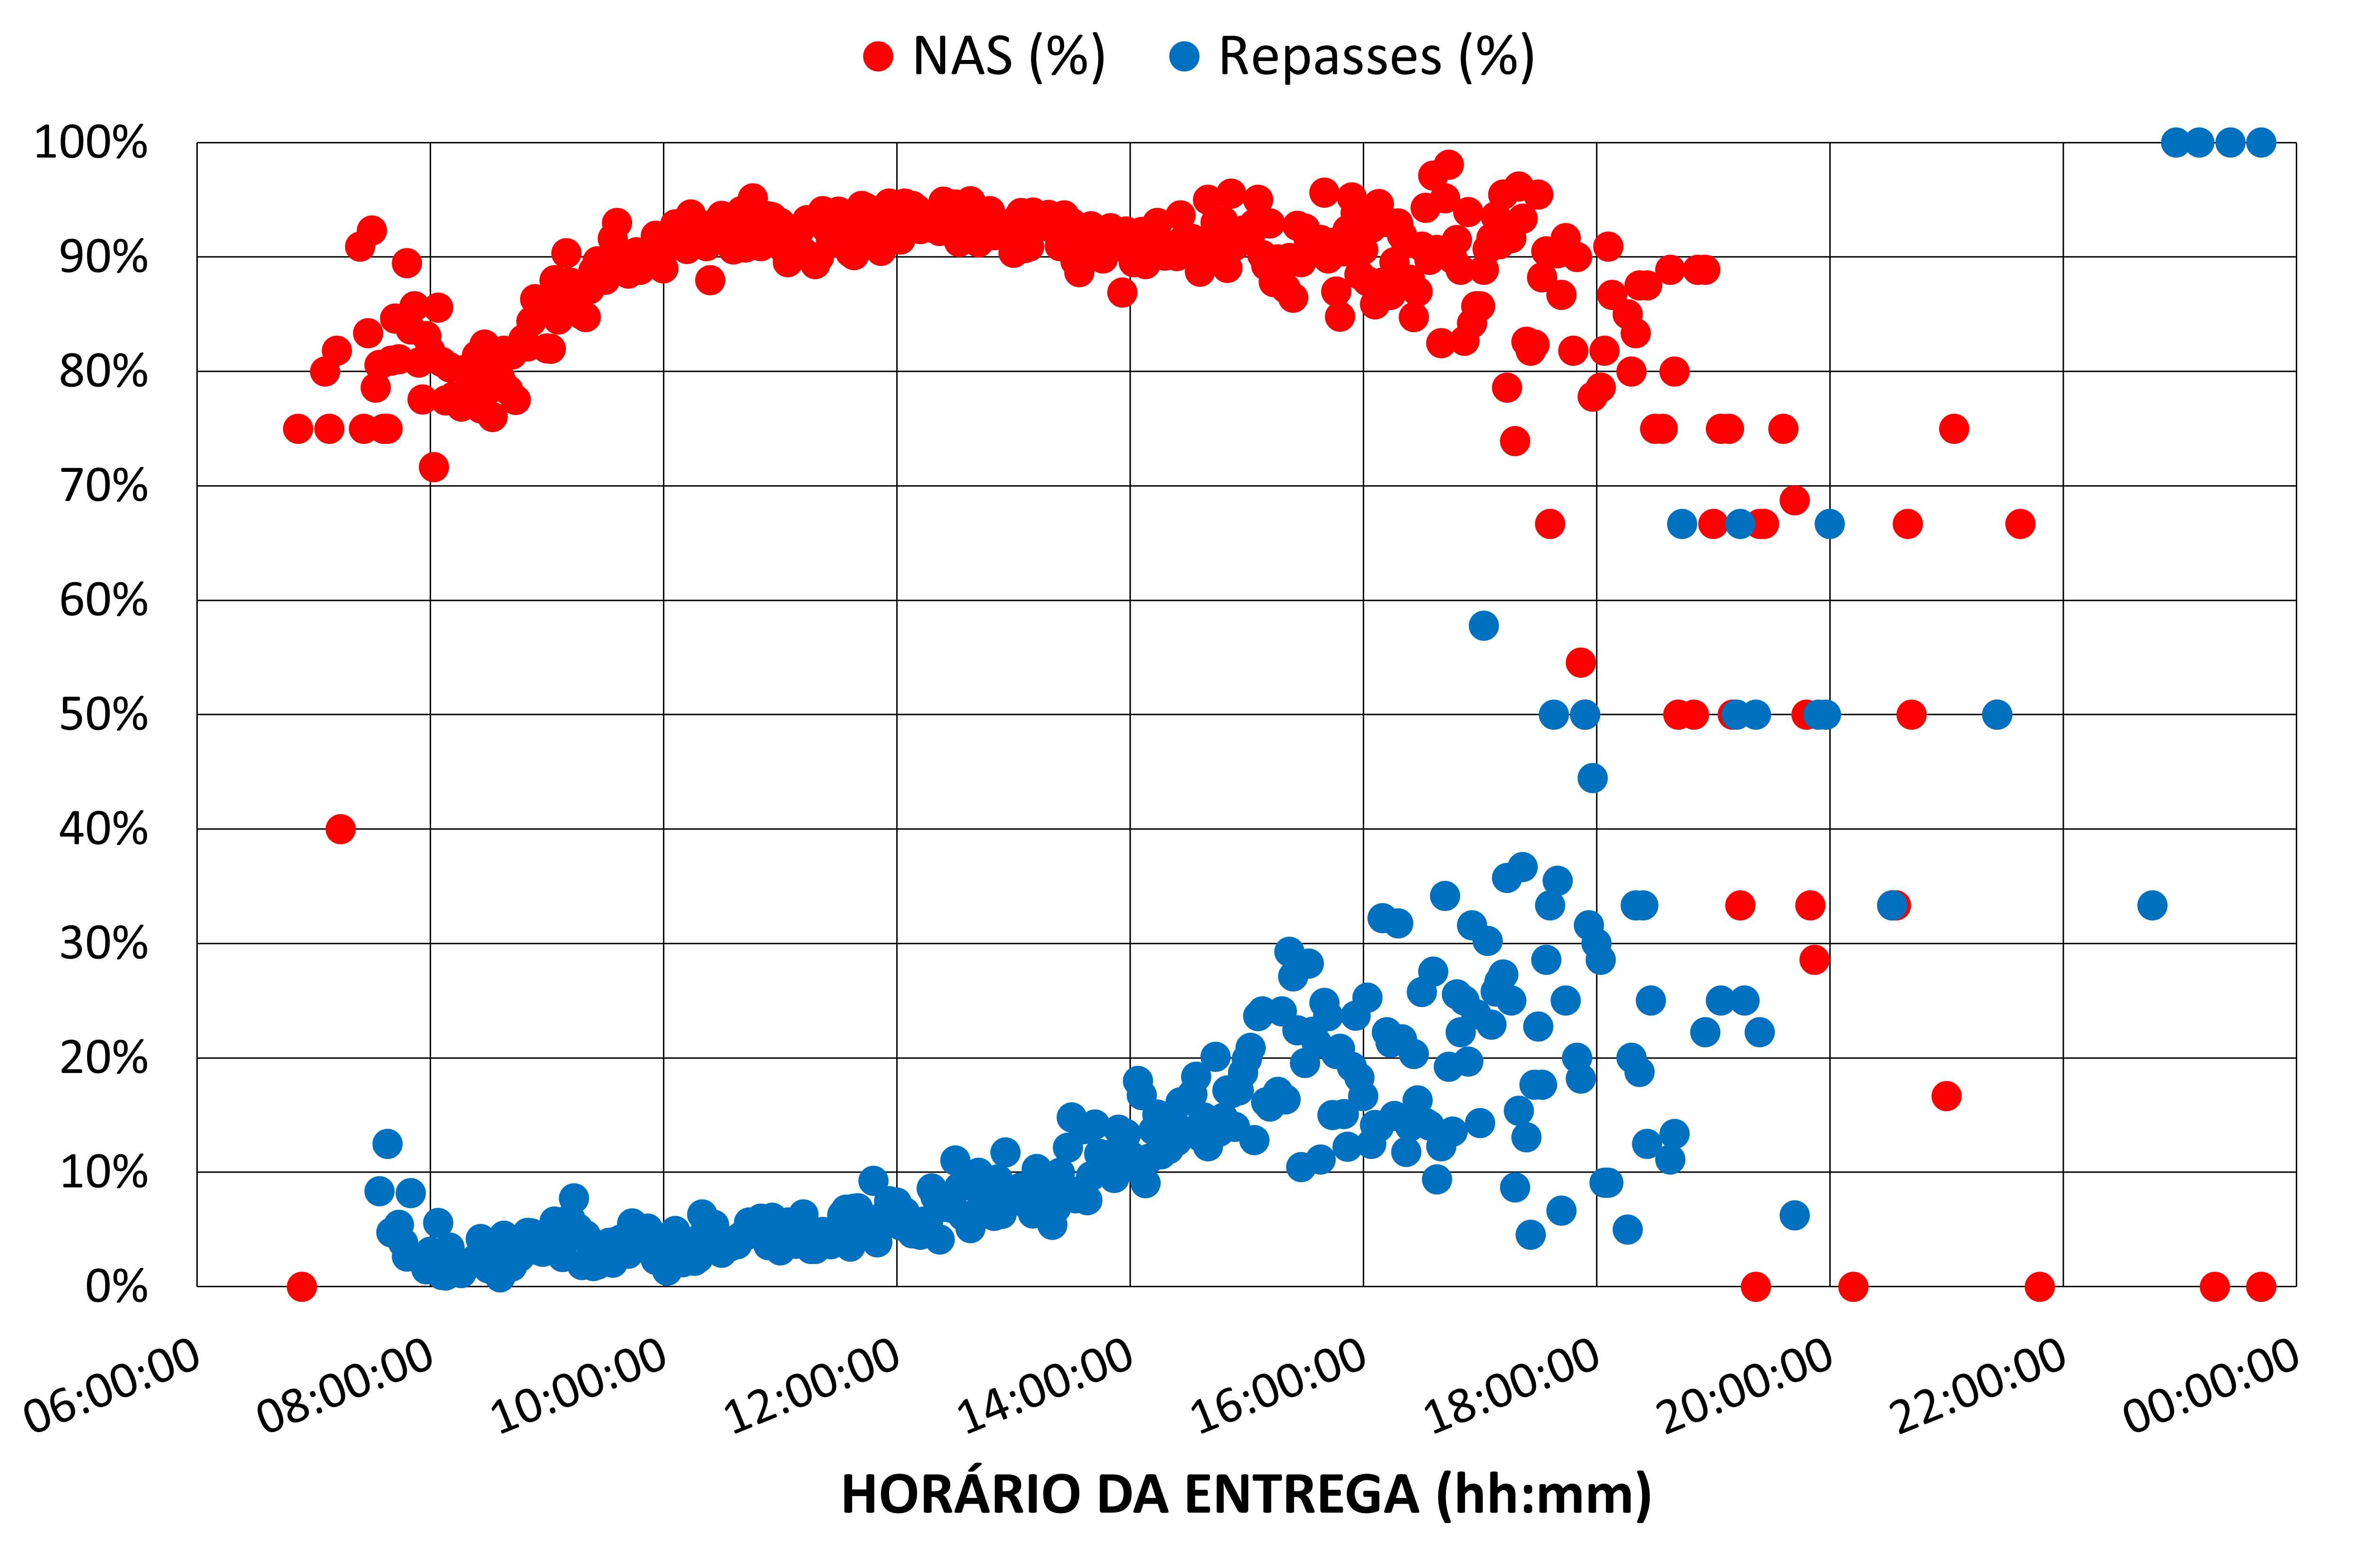
\includegraphics[width=.98\linewidth]{images/5_emp_bebidas/excel_based/Horario.png}
         \label{fig:Horario}
     \end{subfigure}
     \begin{subfigure}{.35\textwidth}
       \centering
       % include second image
       \caption{Estatísticas da Regressão.}
       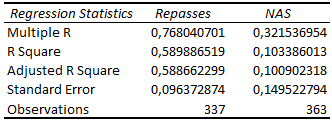
\includegraphics[width=.88\linewidth]{images/5_emp_bebidas/excel_based/Horario_RS.png}
       \label{fig:HorarioRS}
     \end{subfigure}
     \caption*{\ Fonte: Produzido pelos autores Fernandes \& Alves}
 \end{figure} % Horario

Inicialmente, é possível determinar que os primeiros horários do dia são particularmente positivos, apresentando baixos índices de repasses e de NAS. 
Outra informação interessante que pode ser obtida é a de que os horários mais próximos ao almoço (i.e. 11:00 - 13:00) têm maior ocorrência de NAS.
Isso pode ser um indicativo da tendência de alguns clientes ficarem indisponíveis em horários de maior fluxo no setor de restaurantes.
Ademais, isso pode, também, ser um indicativo da tendência da equipe de entregas reajustar seu sequenciamento nas proximidades de sua pausa para almoçar. 
Tal tese, entretanto, pode ser contraposta com a informação adquirida durante visitação presencial de que as equipes em geral tendem a pular o horário de almoço para atingir suas metas e encerrar o horário de trabalho mais cedo.

Por fim, observa-se uma tendência de aumento do volume de repasses ao fim do turno de trabalho. Tal comportamento pode ser explicado pelo costume operacional, identificado na visitação, de se posicionar as revisitas de repasse ao fim do dia.

\subsection{Volume da Entrega}

Também é possível identificar uma variável quantificadora do tamanho de cada entrega que mensura a quantidade de caixas entregues.
Através da visita técnica, verificou-se que a caixa é uma medida padrão estabelecida a partir da garrafeira de entregas média de capacidade de 24 garrafas de 600 ml. 
Outras composições de entregas, tais como os conjuntos de garrafas plásticas de 2 litros ou as latas de alumínio de 350 ml, são convertidas para a unidade de caixas através da equivalência volumétrica.

Intuitivamente, a quantidade de caixas entregues pode apresentar correlação para com as variáveis de repasses e NAS, considerando-se o grau de relevância que a entrega passa a ter para a equipe e o cliente. Assim, volumes maiores a serem entregues podem ser tratados de forma diferente aos volumes menores, o que pode resultar em resultados diferentes entre as variáveis-problema.

Assim, por se tratar de uma variável contínua, foi estabelecida uma análise de correlação através de uma \textit{nuvem de pontos} para cada variável-problema e, em sequência, o destacamento da regressão linear de cada uma.
Nas Figuras \ref{fig:Volume} e \ref{fig:VolumeRS} é possível visualizar essa análise, onde é possível identificar um comportamento de potencial correlação entre o volume entregue e as variáveis.

Cita-se que os cada ponto do gráfico é um PDE. Assim a avaliação é baseada no volume médio recebido por cada PDE no intervalo estudado, assim como seus indicadores de \%REP e \%NAS.

\begin{figure}[H]
     \caption{Correlação entre as variáveis problema e o volume entregue.}
     \begin{subfigure}{.64\textwidth}
         \centering
         % include first image 
         \caption{Relação Gráfica entre as variáveis e o Volume.}
         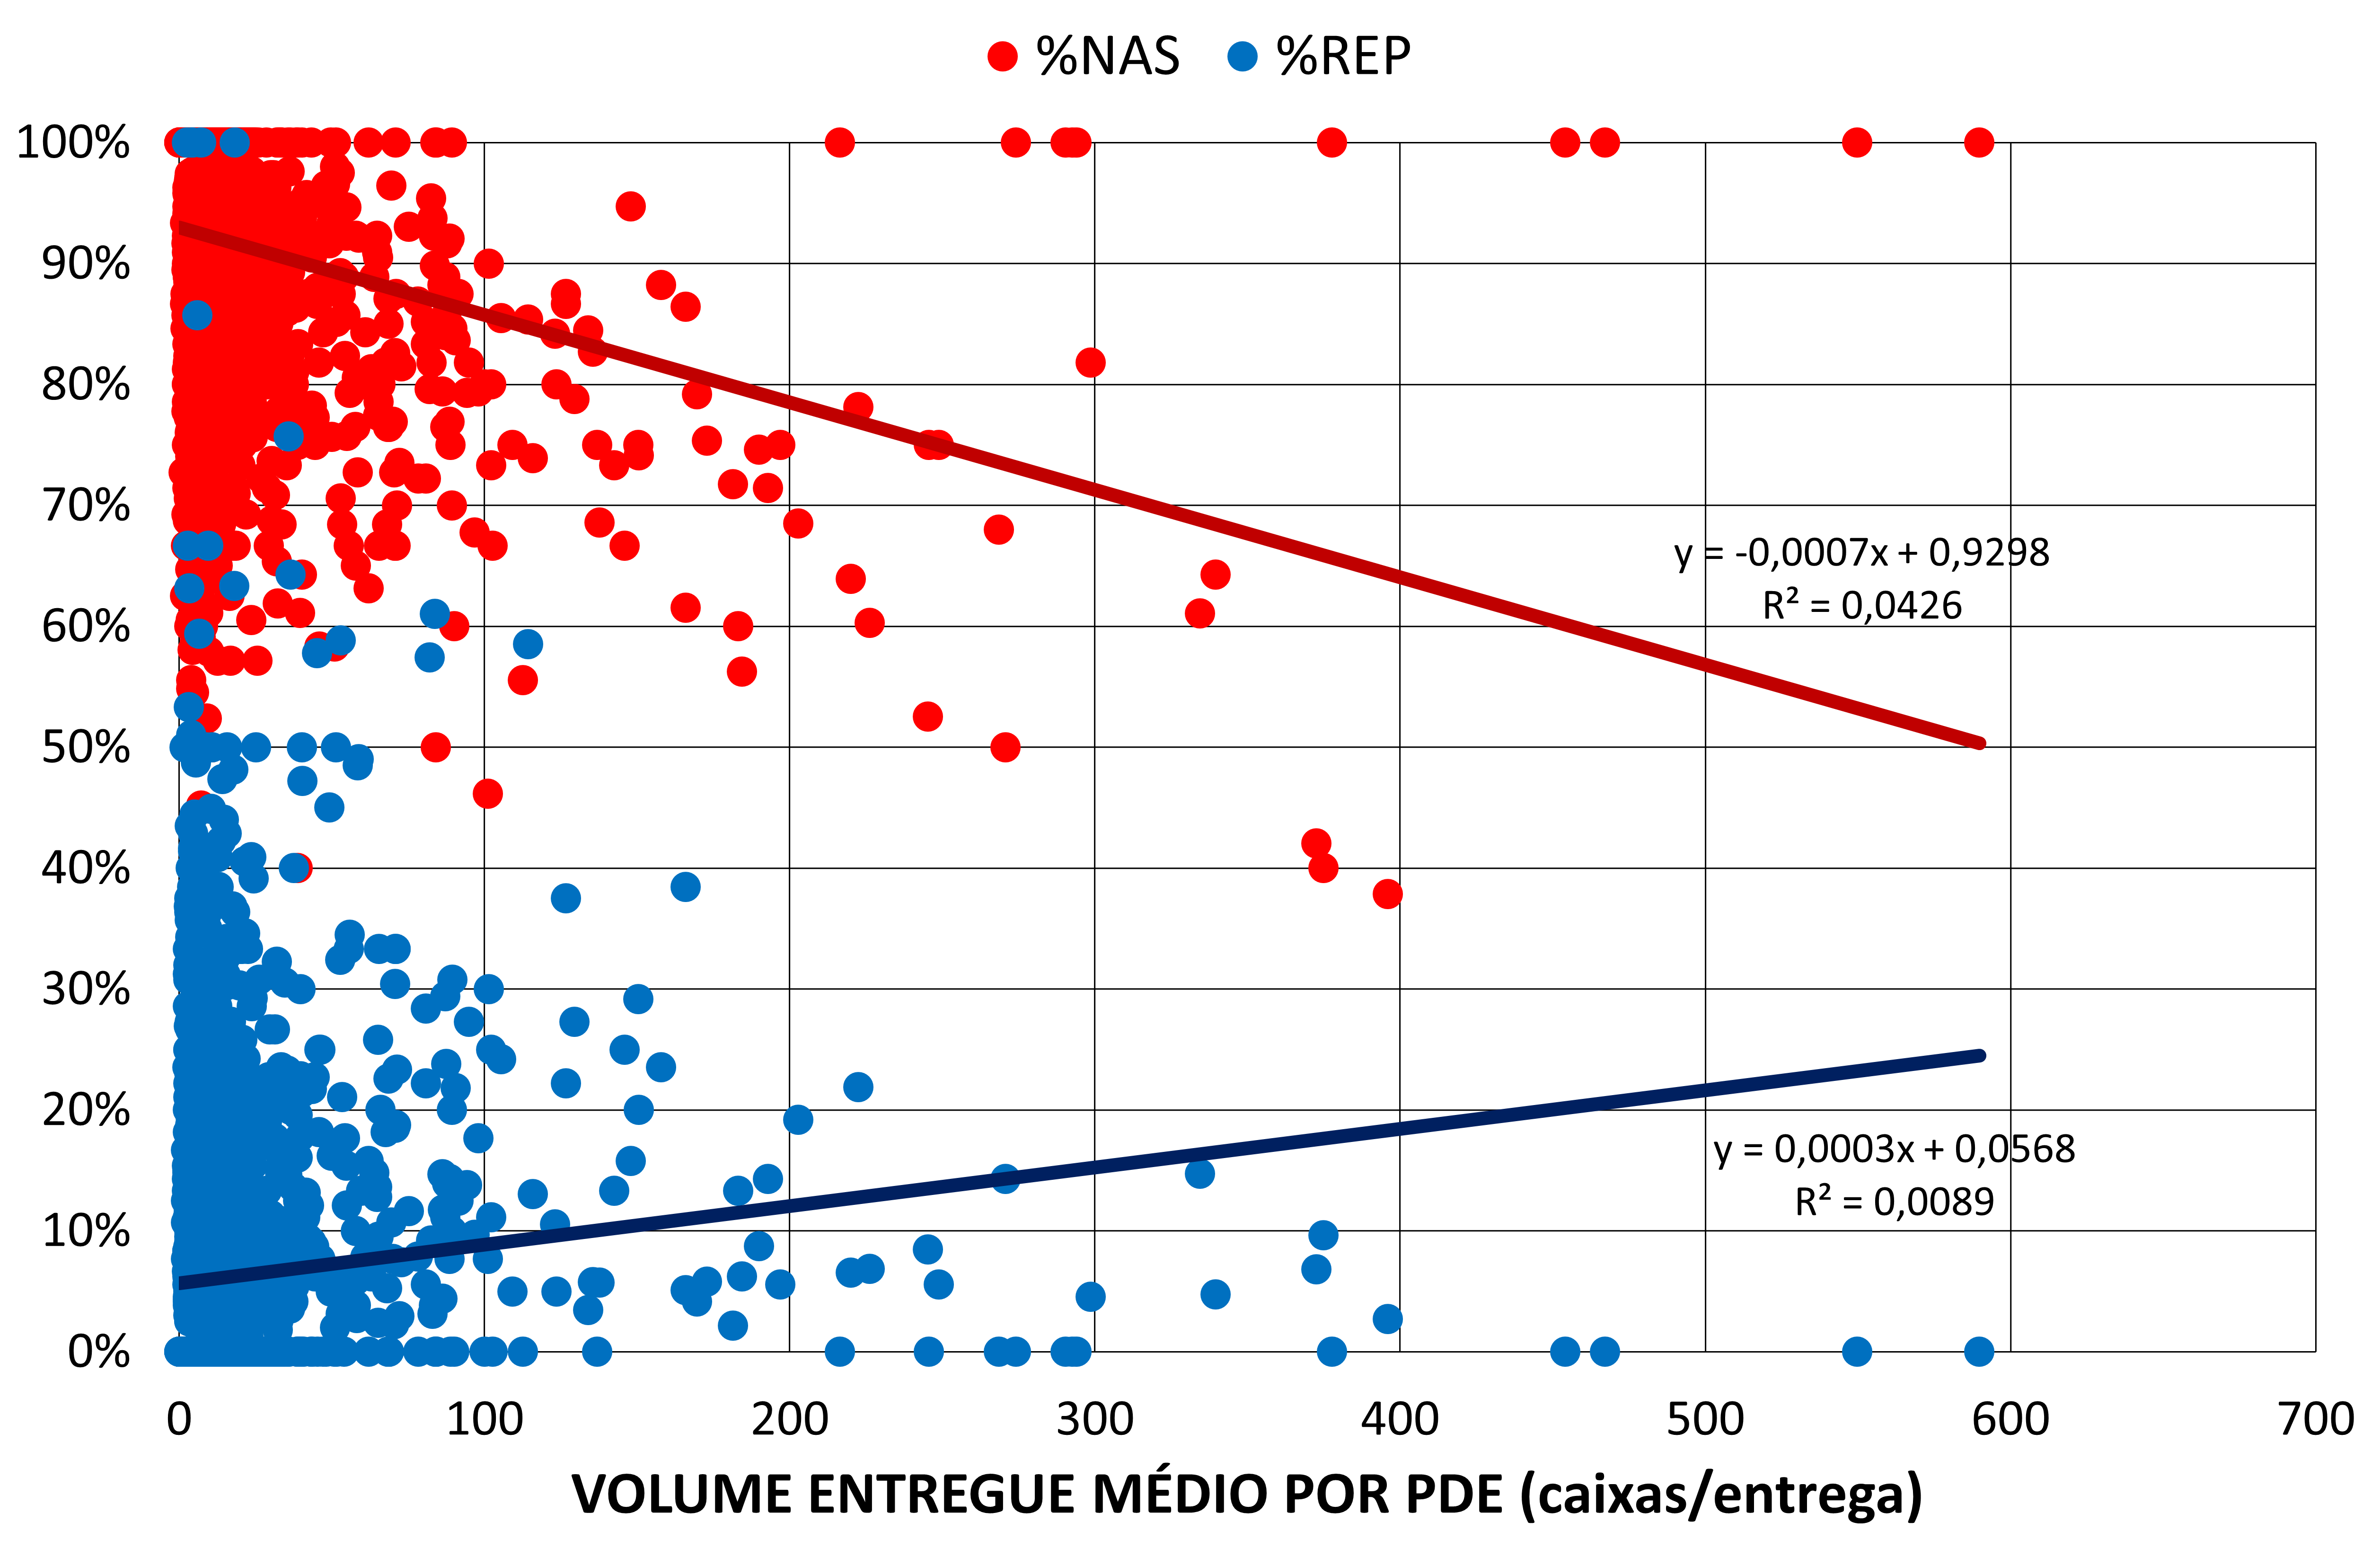
\includegraphics[width=.98\linewidth]{images/5_emp_bebidas/excel_based/Volume.png}
         \label{fig:Volume}
     \end{subfigure}
     \begin{subfigure}{.35\textwidth}
       \centering
       % include second image
       \caption{Estatísticas da Regressão.}
       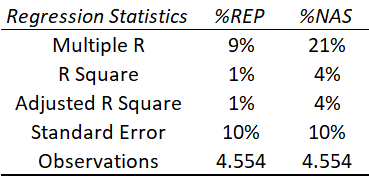
\includegraphics[width=.88\linewidth]{images/5_emp_bebidas/excel_based/Volume_RS.png}
       \label{fig:VolumeRS}
     \end{subfigure}
     \caption*{\ Fonte: Produzido pelos autores Fernandes \& Alves}
\end{figure} % Volume

Observando-se a Figura \ref{fig:Volume} é possível estabelecer que o volume entregue ao PDE tem baixa correlação com os repasses e o NAS. Isso ocorre devido ao alto espalhamento observado dos pontos no gráfico, especialmente em sua porção esquerda, que representa os volumes mais baixos (que são a maioria dos PDE no estudo de caso em questão). Porém, para volumes maiores, é possível observar uma maior padronização na queda de NAS e na queda da ocorrência de repasses, apesar da tendência de regressão dos repasses que é altamente influenciada pelo alto volume de PDE com baixos volumes de entrega com quantidades de repasses percentuais bastante variados.

Tais comportamentos observados para volumes mais altos são coerentes com a concepção de que clientes maiores podem ser tratados com maior cautela pela equipe de entregas, o que leva a uma redução das variáveis-problema.

%%%%%%%%%%%%%%%%%%%%%%%%%%%%%%%%%%%%%%%%%%%%%%%%%%%%%%%%%%%%%%%
\section{Distância entre PDEs e Centro de Distribuição} \label{sec:distanciaCDBebidas}

Em sequência às análises relativas à caracterização da operação da empresa de bebidas, buscou-se identifica-se possíveis efeitos da posição dos PDE nas variáveis problema. Assim, realizou-se a correlação entre os percentuais de repasse, devolução e NAS de cada PDE com sua distância até o CD. 
Foram calculadas as distâncias linear e veicular de todos os PDEs ao CD, considerando toda a base de dados disponível.
Adicionalmente, dispondo-se de ambas as distâncias, calculou-se o fator de circuito para cada par PDE-CD.
Ressalta-se que o processo retrata uma análise preliminar para melhor compreensão das possibilidades de estudo. A posteriori, uma análise mais aprofundada dos efeitos e das diferentes concepções do fator de circuito serão apresentadas na Seção \ref{sec:AMBEV_FC}.

Assim, dispondo-se de todos os indicadores citados, foi possível estabelecer uma correlação entre cada dupla de fatores, conforme ilustrado na Tabela \ref{tab:DistanciaCD_PDEs}, que contém a matriz de correlação entre os diferentes fatores.
Os resultados sugerem que aparentemente não existe uma relação direta entre as variáveis-problema e as distâncias até o CD.
Não obstante, também verifica-se que as três variáveis-problema não possuem relação linear entre si.


\begin{spacing}{1}
\begin{table}[htb] 
    \centering
    \caption{Matriz de correlação entre REP, DEV e NAS e a distância dos PDEs ao CD.}
    \label{tab:DistanciaCD_PDEs}
    % \small
    \begin{tabular}{c|cccccc}
    \hline
    \textit{} & \textit{\%DEV} & \textit{\%NAS} & \textit{\%REP} & \textit{\begin{tabular}[c]{@{}c@{}}Dist Linear\\ CD-PDE\end{tabular}} & \textit{\begin{tabular}[c]{@{}c@{}}Dist Veicular\\ CD-PDE\end{tabular}} & \textit{\begin{tabular}[c]{@{}c@{}}F.C.\\ CD-PDE\end{tabular}} \\ \hline
    \%DEV & \cellcolor[HTML]{63BE7B}1,00 &  &  &  &  &  \\
    \%NAS & \cellcolor[HTML]{FEE883}-0,02 & \cellcolor[HTML]{63BE7B}1,00 &  &  &  &  \\
    \%REP & \cellcolor[HTML]{ECE683}0,11 & \cellcolor[HTML]{FED980}-0,06 & \cellcolor[HTML]{63BE7B}1,00 &  &  &  \\
    Dist Linear CD-PDE & \cellcolor[HTML]{FEE382}-0,04 & \cellcolor[HTML]{EFE784}0,09 & \cellcolor[HTML]{FEDC81}-0,06 & \cellcolor[HTML]{63BE7B}1,00 &  &  \\
    Dist Veicular CD-PDE & \cellcolor[HTML]{FEDC81}-0,06 & \cellcolor[HTML]{EDE683}0,10 & \cellcolor[HTML]{FDD780}-0,07 & \cellcolor[HTML]{71C37C}0,91 & \cellcolor[HTML]{63BE7B}1,00 &  \\
    F.C. CD-PDE & \cellcolor[HTML]{FEE883}-0,03 & \cellcolor[HTML]{FEDE81}-0,05 & \cellcolor[HTML]{FFEB84}-0,02 & \cellcolor[HTML]{F8696B}-0,36 & \cellcolor[HTML]{FCC47C}-0,12 & \cellcolor[HTML]{63BE7B}1,00 \\ \hline
    \end{tabular}
    % \normmalsize
    \caption*{Fonte: Produzido pelos autores Fernandes \& Alves}
\end{table}
\end{spacing}

%%%%%%%%%%%%%%%%%%%%%%%%%%%%%%%%%%%%%%%%%%%%%%%%%%%%%%%%%%%%%%%
\section{Dispersão geográfica das rotas} \label{sec:dispersaoBebidas}

Ainda considerando a posição geográfica dos PDE, busca-se compreender de forma mais ampla como que o conjunto de clientes englobados numa mesma rota podem variar suas taxas de repasse, devolução e NAS a partir de suas dispersões geográficas.

Primeiramente, utilizando o modelo descrito na seção \ref{sec:dispGeoRotas}, calcula-se o conjunto de PDEs considerados ``muito distantes'' dentro de cada rota. 
Isto é, aqueles PDEs que estão localizados fora da ``cauda'' de uma distribuição normal que represente a distribuição das coordenadas dos PDEs, considerando 5\% de significância. 

Em seguida, calculou-se os parâmetros percentuais de repasses, devoluções e NAS para os pontos dentro e fora da região da ``cauda'' e replicou-se o método inteiro para distâncias lineares e veiculares. 
Por fim, os resultados obtidos podem ser observados na Tabela \ref{tab:CompactacaoRotas}, a partir dos quais é possível estabelecer que os PDEs localizados à margem de suas rotas não apresentam resultados consideravelmente distintos daqueles não marginalizados.
Ademais, comparando-se os resultados de ambas distâncias, observa-se pouca variação entre a linear e a veicular.

Em destaque, pode-se considerar a variação no percentual de NAS entre os pontos marginais e os não marginais.
Tal resultado é coerente com a ideia de que a equipe de entrega pode ser mais cautelosa com os PDEs mais distantes de sua rota, devido ao maior consumo de tempo que sua visita exige, evitando-se, assim, alterações da posição sequencial a esmo dos PDEs em questão.

\begin{spacing}{1}
\begin{table}[htb] 
    \centering
    \caption{Resultados da avaliação de PDEs localizados à margem de suas rotas.}
    \label{tab:CompactacaoRotas}
    \begin{tabular}{cccc}
    \hline
    \rowcolor[HTML]{4472C4} 
    \multicolumn{1}{|c|}{\cellcolor[HTML]{548235}{\color[HTML]{FFFFFF} Distância  Linear}} & \multicolumn{1}{c|}{\cellcolor[HTML]{4472C4}{\color[HTML]{FFFFFF} \%REP}} & \multicolumn{1}{c|}{\cellcolor[HTML]{4472C4}{\color[HTML]{FFFFFF} \%DEV}} & \multicolumn{1}{c|}{\cellcolor[HTML]{4472C4}{\color[HTML]{FFFFFF} \%NAS}} \\ \hline
    \multicolumn{1}{|c|}{Fora da Cauda} & \multicolumn{1}{c|}{7\%} & \multicolumn{1}{c|}{2\%} & \multicolumn{1}{c|}{94\%} \\ \hline
    \multicolumn{1}{|c|}{Dentro da Cauda} & \multicolumn{1}{c|}{8\%} & \multicolumn{1}{c|}{1\%} & \multicolumn{1}{c|}{90\%} \\ \hline
    \multicolumn{1}{l}{} & \multicolumn{1}{l}{} & \multicolumn{1}{l}{} & \multicolumn{1}{l}{} \\ \hline
    \rowcolor[HTML]{4472C4} 
    \multicolumn{1}{|c|}{\cellcolor[HTML]{BF8F00}{\color[HTML]{FFFFFF} Distância Veicular}} & \multicolumn{1}{c|}{\cellcolor[HTML]{4472C4}{\color[HTML]{FFFFFF} \%REP}} & \multicolumn{1}{c|}{\cellcolor[HTML]{4472C4}{\color[HTML]{FFFFFF} \%DEV}} & \multicolumn{1}{c|}{\cellcolor[HTML]{4472C4}{\color[HTML]{FFFFFF} \%NAS}} \\ \hline
    \multicolumn{1}{|c|}{Fora da Cauda} & \multicolumn{1}{c|}{7\%} & \multicolumn{1}{c|}{2\%} & \multicolumn{1}{c|}{94\%} \\ \hline
    \multicolumn{1}{|c|}{Dentro da Cauda} & \multicolumn{1}{c|}{8\%} & \multicolumn{1}{c|}{1\%} & \multicolumn{1}{c|}{91\%} \\ \hline
    \end{tabular}
    \caption*{Fonte: Produzido pelos autores Fernandes \& Alves}
\end{table}
\end{spacing}

%%%%%%%%%%%%%%%%%%%%%%%%%%%%%%%%%%%%%%%%%%%%%%%%%%%%%%%%%%%%%%%
\section{Geoestatísticas} \label{sec:geoestatBebidas}

Posteriormente às análises de posicionamento relativo dos PDE, buscou-se, na presente seção, estabelecer um conjunto de análises geoestatísticas a partir da base de dados da empresa de bebidas a fim de se compreender se existe alguma tendência geográfica em ampla escala entre as variáveis-problema estudadas.
Essa análise contemplou apenas a cidade de Guarulhos, que representa 80\% do total de entregas disponíveis na base de dados da empresa de bebidas.

As análises construídas na presente seção são realizadas através da ferramenta GeoDa, cujo uso foi descrito com maiore detalhamento em \ref{GeoDa}. Os conceitos e teorias por trás das análises realizadas, assim como uma apresentação formal dos indicadores representados, pode ser encontrada em \ref{sec:autocorrelacaoEsp}.

Os resultados, que podem ser observados nas Figuras de \ref{fig:AMBEV_LISA_REP} até %, \ref{fig:AMBEV_SCT_REP}, \ref{fig:AMBEV_LISA_DEV}, \ref{fig:AMBEV_SCT_DEV}, \ref{fig:AMBEV_LISA_NAS} e 
\ref{fig:AMBEV_SCT_NAS}, indicam baixa tendência de correlação espacial entre as variáveis estudadas e os bairros da cidade. 
Como observa-se nos três mapas LISA, a maioria dos bairros enquadrou-se como não relevantes (cinza), ou seja, não se pode identificar um padrão espacial na disposição dos clientes que tiveram repasse, devolução ou NAS. 
Este fato é corroborado com o gráfico de dispersão. 
Pode-se observar nos três gráficos apresentados (\ref{fig:AMBEV_SCT_REP}, \ref{fig:AMBEV_SCT_DEV} e \ref{fig:AMBEV_SCT_NAS}) que a correlação estabelecida é numericamente reduzida.

Comparando-se os resultados entre si é possível afirmar que as devoluções e o NAS apresentaram os resultados mais promissores e, nas análises subsequentes, poderão conduzir a resultados mais robustos. 
Tal conclusão é coerente com a percepção de que os repasses podem estar, proporcionalmente, mais associados a comportamentos e decisões dos clientes e da equipe de entregas do que o NAS.% que teve o maior índice de correlação espacial.

\begin{figure}[htb]
     \caption{Correlação espacial do percentual de repasses por bairro.}
     \begin{subfigure}{.49\textwidth}
         \centering
         \caption{Mapa LISA.}
         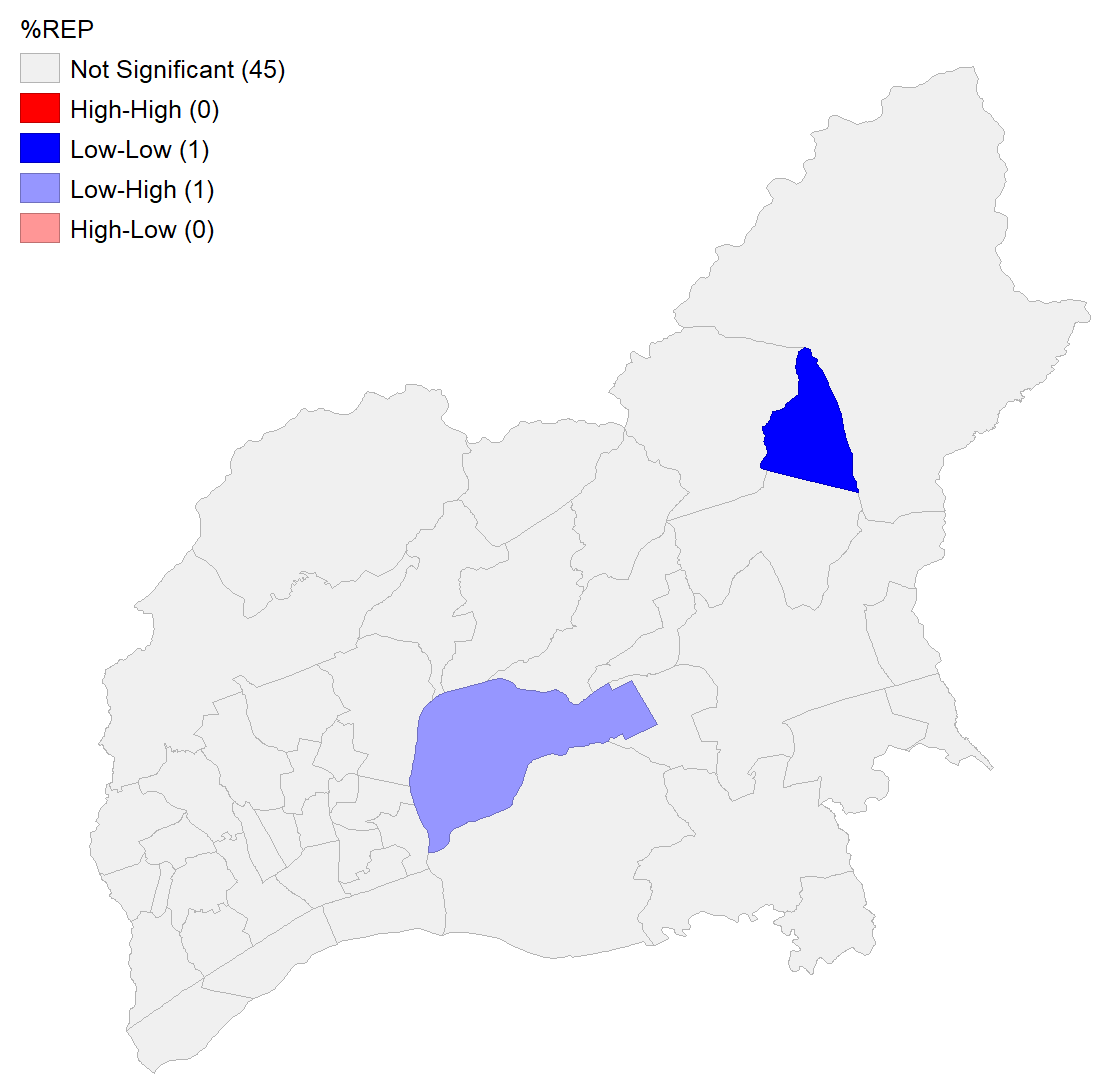
\includegraphics[height=0.75\textwidth]{images/5_emp_bebidas/geoda/BairrosOSM_Corrigidos_REP_lisa.png}
         \label{fig:AMBEV_LISA_REP}
     \end{subfigure}
     \begin{subfigure}{.49\textwidth}
       \centering
       % include second image
       \caption{Gráfico de Dispersão.}
       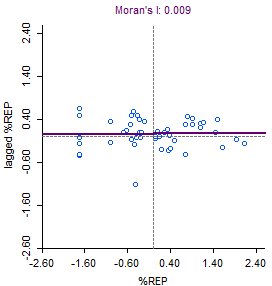
\includegraphics[height=0.75\textwidth]{images/5_emp_bebidas/geoda/BairrosOSM_Corrigidos_REP_sct.png}
       \label{fig:AMBEV_SCT_REP}
     \end{subfigure}
     \caption*{\ Fonte: Produzido pelos autores Fernandes \& Alves}
 \end{figure} % Repasses

\begin{figure}[htb]
     \caption{Correlação espacial do percentual de devoluções por bairro.}
     \begin{subfigure}{.49\textwidth}
         \centering
         % include first image 
         \caption{Mapa LISA.}
         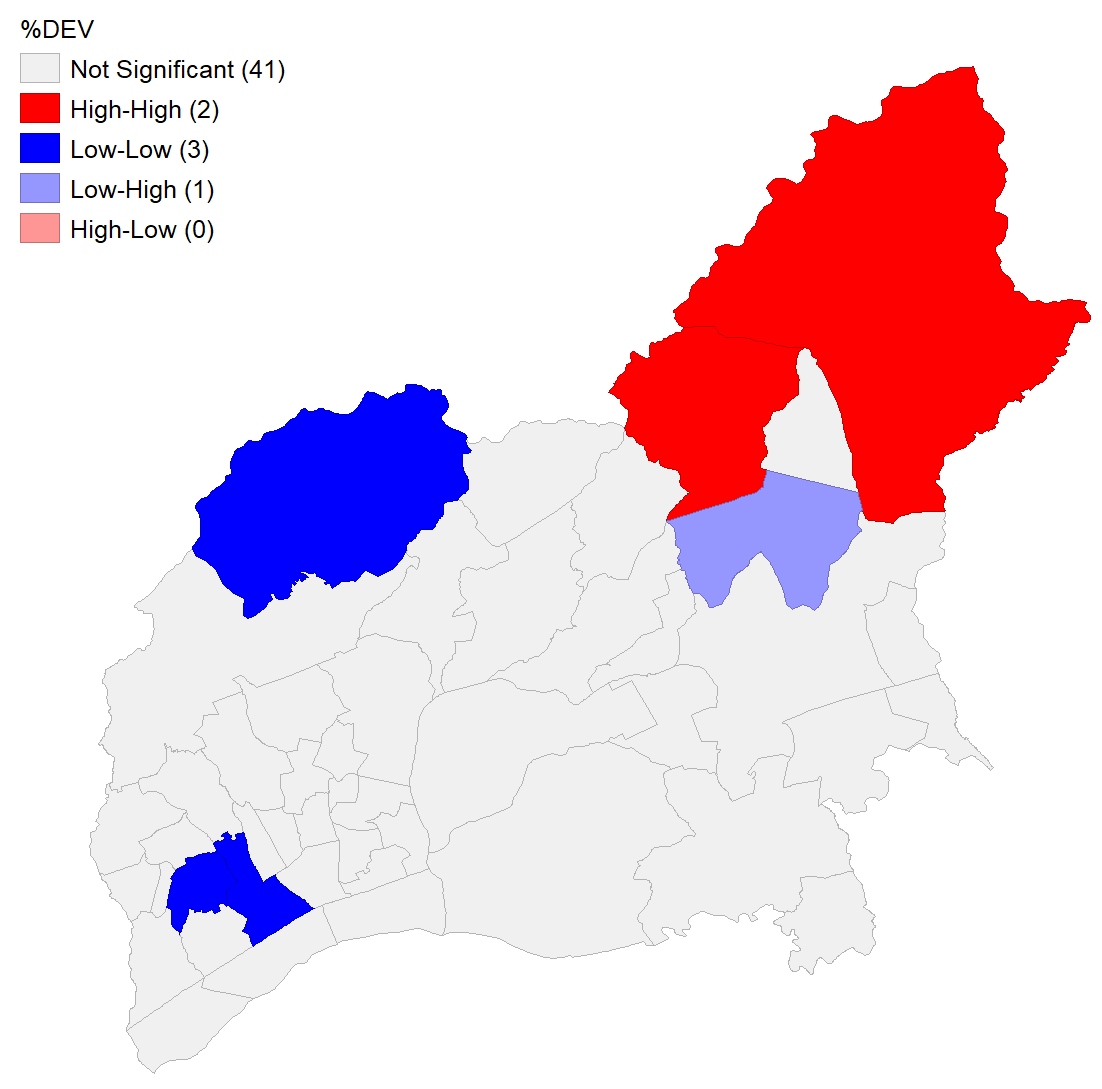
\includegraphics[height=0.75\textwidth]{images/5_emp_bebidas/geoda/BairrosOSM_Corrigidos_DEV_lisa.png}
         \label{fig:AMBEV_LISA_DEV}
     \end{subfigure}
     \begin{subfigure}{.49\textwidth}
       \centering
       % include second image
       \caption{Gráfico de Dispersão.}
       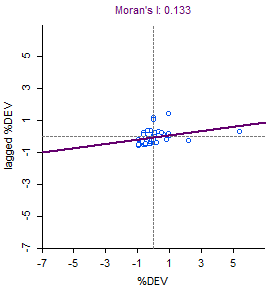
\includegraphics[height=0.75\textwidth]{images/5_emp_bebidas/geoda/BairrosOSM_Corrigidos_DEV_sct.png}
       \label{fig:AMBEV_SCT_DEV}
     \end{subfigure}
     \caption*{\ Fonte: Produzido pelos autores Fernandes \& Alves}
 \end{figure} % Devoluções

\begin{figure}[htb]
     \caption{Correlação espacial do percentual de NAS por bairro.}
     \begin{subfigure}{.49\textwidth}
         \centering
         % include first image 
         \caption{Mapa LISA.}
         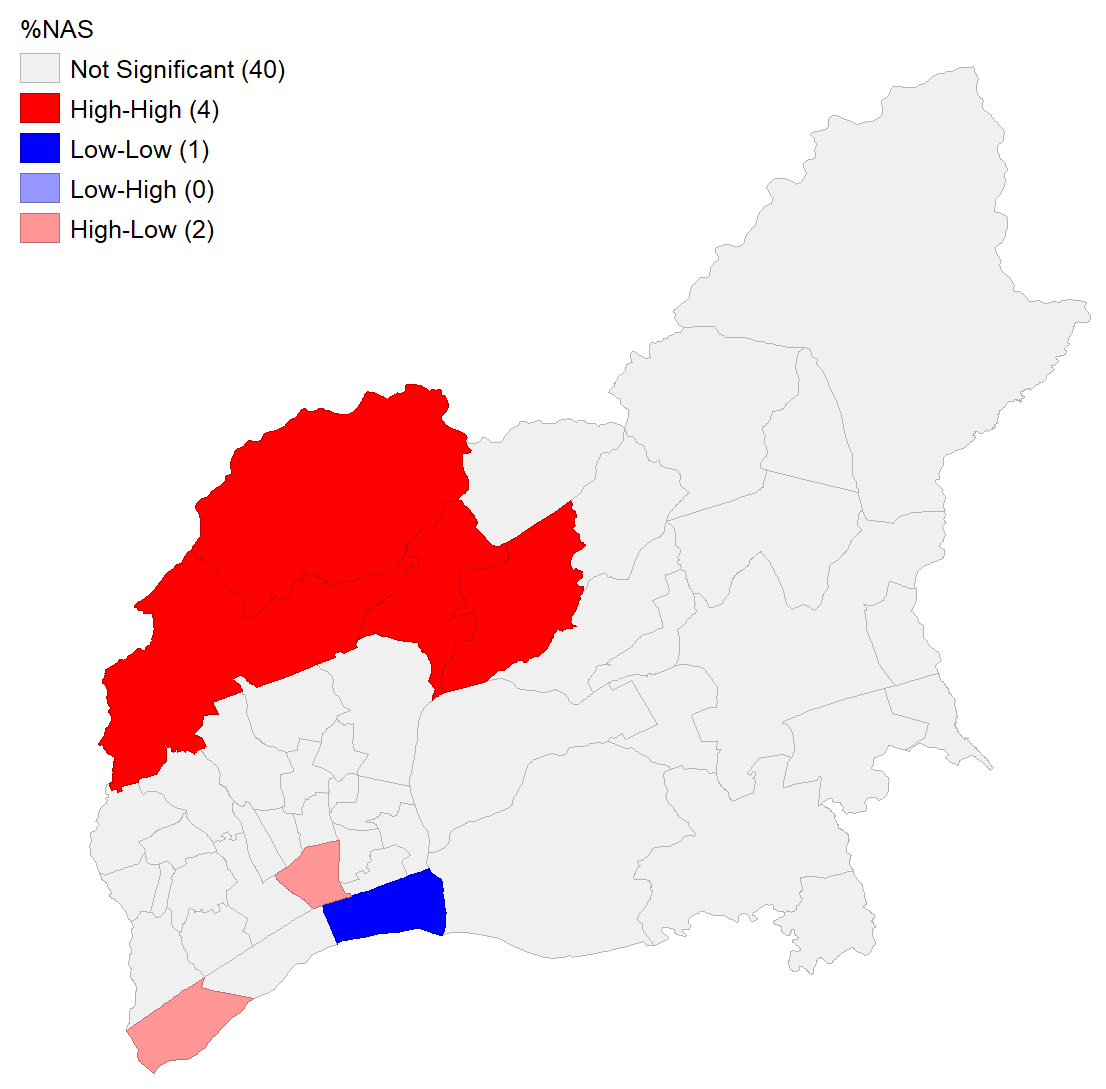
\includegraphics[height=0.75\textwidth]{images/5_emp_bebidas/geoda/BairrosOSM_Corrigidos_NAS_lisa.png}
         \label{fig:AMBEV_LISA_NAS}
     \end{subfigure}
     \begin{subfigure}{.49\textwidth}
       \centering
       % include second image
       \caption{Gráfico de Dispersão.}
       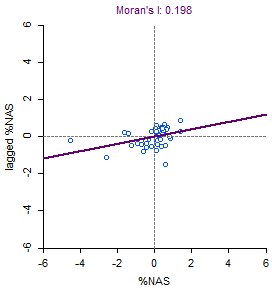
\includegraphics[height=0.75\textwidth]{images/5_emp_bebidas/geoda/BairrosOSM_Corrigidos_NAS_sct.png}
       \label{fig:AMBEV_SCT_NAS}
     \end{subfigure}
     \caption*{\ Fonte: Produzido pelos autores Fernandes \& Alves}
 \end{figure} % NAS

A análise de correlação espacial, porém, não é determinística acerca da possibilidade de haver alguma relação espacial entre os dados, ela se resume, apenas, a um teste de agrupamento entre vizinhos.
Assim, ainda é possível avaliar outros aspectos da localização dos clientes, tal como a influência da estrutura viária dos arredores e das rotas nas variáveis-problema.

%%%%%%%%%%%%%%%%%%%%%%%%%%%%%%%%%%%%%%%%%%%%%%%%%%%%%%%%%%%%%%%
\section{Fator de circuito} \label{sec:AMBEV_FC}

%%%%%%%%%%%%%%%%%%%%%%%%%%%%%%%%%%%%%%%%%%%%%%%%%%%%
\subsection{Validação do modelo}

Antes de partir para o cálculo do fator de circuito envolvendo toda a malha viária estudada, optou-se por selecionar arbitrariamente um PDE que apresentasse alta taxa de repasses e então utilizá-lo como ponto de origem para realização dos cálculos de fator de circuito considerando diferentes pontos ao redor deste PDE e inseridos em um quadrado de lado igual a dois quilômetros.
%
A Figura \ref{fig:FC_1ponto} apresenta o resultado obtido, onde em geral nota-se a presença de uma segmentação dos valores de fator de circuito em relação à região estudada. 
Ou seja, quando o ponto de destino passa a estar localizado em regiões mais ao sudeste da imagem, região essa especialmente separada da parte norte por uma via transversal de grande porte (no caso a Rodovia Presidente Dutra, principal rodovia que atravessa a cidade), os valores de fator de circuito tendem a aumentar.
%

Deste modo fica comprovada a influência que alguns elementos da malha viária podem exercer sobre a medida de fator de circuito, permitindo que as demais análises do trabalho investiguem se essa relação pode ser estendida para medidas tais como a quantidade de repasses e NAS, conforme será apresentado posteriormente.

Para além dos efeitos da Rodovia Presidente Dutra, é interessante que se estabeleça uma visualização mais integrada entre o espaço físico e os resultados de fator de circuito em relação ao ponto em questão.
Para tal, considerou-se a construção de isolinhas - ou linhas de contorno - da medida fator de circuito. 

A Figura \ref{fig:FC_1ponto_iso} apresenta as linhas de contorno em intervalo de 0,5 para o fator de circuito.
É possível evidenciar ainda mais o efeito da rodovia Presidente Dutra sobre os valores de fator de circuito.
Quando observado mais à esquerda, onde há um acesso bem estabelecido, os valores aproximam-se de 3 ao sul da rodovia.
Contudo, na região mais à direita, que conta com menos acessos diretos à rodovia, o valor do fator de circuito pode chegar a 7, novamente ao sul da rodovia. 

Ademais, destaca-se que o fator de circuito nas proximidades do ponto estudado possui valores maiores do que nas extremidades do quadrado analisado, exemplificando o fenômeno descrito pela Equação \ref{eq:limite}. 

Sendo assim, é possível considerar que uma barreira física, como é o caso da rodovia Presidente Dutra, pode apresentar um impacto significativo na ``circuicidade'' da região estudada, reforçando que a geometria da malha viária pode afetar a facilidade de entregas de última milha.

\begin{figure}[H]
    \centering
    \caption{Fator de circuito ao redor de um PDE selecionado}
    \includegraphics[width=0.8\textwidth]{images/5_emp_bebidas/qgis/ResultadoPreliminarQGIS 1.4.pdf}
    \caption*{\ Fonte: Produzido pelos autores Fernandes \& Alves}
    \label{fig:FC_1ponto}
\end{figure}

\begin{figure}[H]
    \centering
    \caption{Isolinhas do fator de circuito ao redor de um PDE selecionado}
    \includegraphics[width=0.8\textwidth]{images/5_emp_bebidas/qgis/ResultadoPreliminarQGIS 1.10.png}
    \caption*{\ Fonte: Produzido pelos autores Fernandes \& Alves}
    \label{fig:FC_1ponto_iso}
\end{figure}

%%%%%%%%%%%%%%%%%%%%%%%%%%%%%%
\subsection{Resultados gerais}

Uma vez evidenciada a interferência entre fator de circuito e malha viária, é possível utilizar dos códigos descritos no capítulo \ref{sec:mat&met} para realizar consultas de distâncias veiculares através do \textit{Google Maps API} e assim avaliar o fator de circuito inserido no contexto da presente pesquisa.

Para realizar os cálculos de fator de circuito, considera-se cada trecho que possa ter sido percorrido por ao menos um veículo. 
Isto inclui os trechos que partem do CD até os PDEs e também os que saem dos PDEs até os PDEs seguintes.
Ao todo, um total de 61.778 trechos tiveram que ser computados em termos de distância euclidiana e veicular, assim como do fator de circuito.
Deste modo, são aplicados os métodos descritos no capítulo \ref{sec:mat&met}, com auxílio da biblioteca \textit{lmr\_analyzer}, os resultados são exportados e puderam então ser analisados.

Tendo posse dos resultados de fator de circuito, foi possível utilizar o \textit{software} QGIS para representar a distribuição espacial dos elementos da matriz de distância, conforme apresentado na Figura \ref{fig:FC_maps2}. 
A Figura mostra o fator de circuito entre diferentes PDEs, filtrados somente aqueles em que a distância não é superior a 500 metros. 
% 
Tal consideração se dá pela relação percebida entre o valor de circuito e a distância real, uma vez que para distâncias grandes o fator de circuito tende a ser cada vez mais próximo de 1.
%
Sendo assim, alternativamente, filtra-se os dados de modo a apresentar somente os casos em que a distância em linha reta entre dois pontos seja de aproximadamente 500 metros, como pode ser visto na Figura . 
%
A distância de 500 metros foi escolhida com base na literatura (\citeauthoronline{AMARAL2020102916}, \citeyear{AMARAL2020102916}). 
%
A Figura \ref{fig:FC_maps3} apresenta um ponto focal da Figura \ref{fig:FC_maps2}. 

\begin{figure}[H]
    \centering
    \caption{Fator de circuito obtido através do \textit{Google Maps} filtrados para distâncias de até 500 metros }
    \includegraphics[width=0.8\textwidth]{images/5_emp_bebidas/qgis/ResultadoPreliminarQGIS 1.6.pdf}
    \caption*{\ Fonte: Produzido pelos autores Fernandes \& Alves}
    \label{fig:FC_maps2}
\end{figure}

\begin{figure}[H]
    \centering
    \caption{Fator de circuito obtido através do \textit{Google Maps} filtrados para distâncias de até 500 metros, com destaque para região próxima ao CD}
    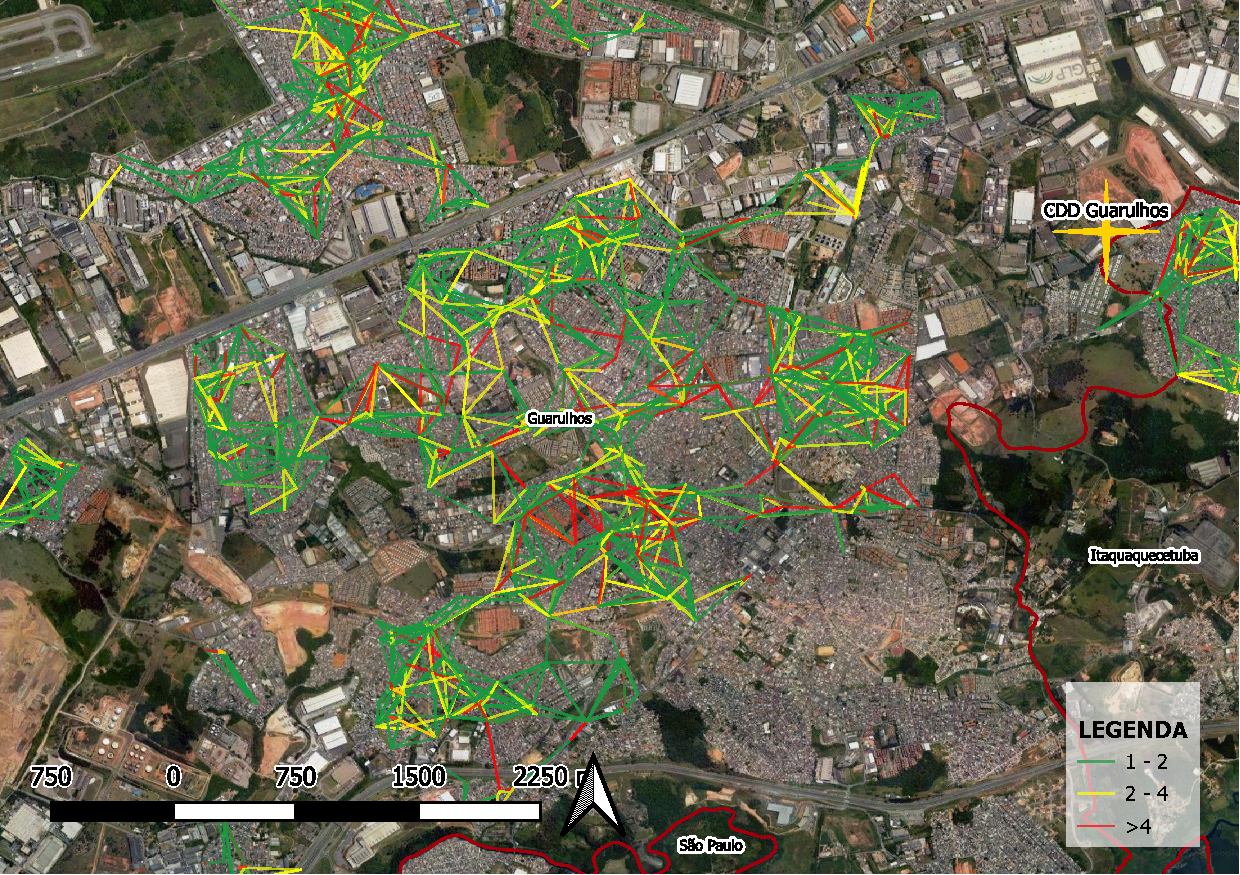
\includegraphics[width=0.8\textwidth]{images/5_emp_bebidas/qgis/ResultadoPreliminarQGIS 1.7.pdf}
    \caption*{\ Fonte: Produzido pelos autores Fernandes \& Alves}
    \label{fig:FC_maps3}
\end{figure}


%%%%%%%%%%%%%%%%%%%%%%%%%%%%%%%%%%%%%%%%%%%%%%%%%%%%%%%%%%%%%%%
\section{Análise da Malha viária} \label{sec:AMBEV_MalhaViaria}

Na presente seção foi descrita a última parte das análises realizadas para o estudo de caso da empresa de bebidas, onde serão aplicados os métodos introduzidos no capítulo \ref{sec:mat&met} para quantificar a topologia da malha viária para cada um dos bairros da cidade de Guarulhos, que é a cidade que compreende a maior região de interesse do estudo (cerca de 80\% da entregadas observadas estão em Guarulhos).
Inicialmente foi testado o modelo para um dos bairros, escolhido aleatoriamente. 
E em seguida foi expandida a análise para todos os demais bairros presentes na cidade.

%%%%%%%%%%%%%%%%%%%%%%%%%%%%%%%%%%%%%%%%%%%%%%%%%%%%%%%%%%
\subsection{Exemplo de aplicação para o bairro de Cumbica}

A partir do arquivo \textit{shapefile} de Guarulhos, utiliza-se um filtro para selecionar apenas o bairro de Cumbica, que será o objeto de estudo desta subseção. 
%
A Figura \ref{fig:Cumbica_network_example} ilustra o conjunto de nós e arcos que representa o bairro de Cumbica, resultado do processo descrito até aqui.
%

Também é possível estudar a problemática de conectividade dos nós da malha conforme descrito por \citeonline{boeing2019urban}, a fim de entender a distribuição espacial da conectividade desses nós.
%
A Figura \ref{fig:network_centrality_cumbica} apresenta o resultado obtido para o bairro de Cumbica, em que os nós mais claros representam uma maior conectividade, ou seja, uma maior quantidade de vias partindo ou chegando dos nós centrais quando comparado com os nós mais periféricos. 

Ademais, as Figuras \ref{fig:Cumbica_bearing_example_histogram} e \ref{fig:Cumbica_bearing_example_polarplot} ilustram o resultado obtido para a análise de orientação de vias - descrita no capítulo \ref{sec:mat&met}, onde cada barra representa um intervalo de $10^{\circ}$.
Em geral nota-se que o bairro de Cumbica tem uma predominância de vias orientadas na direção $50^{\circ}-230^{\circ}$.

Finalmente, é possível gerar e exportar resultados de estatísticas discretas sobre a malha através dos métodos disponíveis na biblioteca \textit{lmr\_analyzier}, já descritos no capítulo \ref{sec:mat&met}.
%
Uma descrição completa das estatísticas obtidas está apresentada no capítulo de apêndice \ref{sec:appResultMalha}, uma vez que consumiriam demasiado tempo de leitura sendo que não são necessariamente cruciais para entendimento do texto. 
Ademais, uma descrição mais resumida dos resultados será apresentada ainda neste capítulo, na seção \ref{sec:relMetricasBebidas}.

Nesta subseção foram calculadas medidas relativas à orientação de vias, conectividade de nós e parâmetros gerais da malha viária de Cumbica, Guarulhos, assim permitindo validar o modelo e testar algumas das ferramentas na prática.
%
Uma vez que se obtém a validação para um dos importantes bairros da amostra de estudo, podendo finalmente prosseguir para a análise global considerando todos os bairros disponíveis. 

\begin{figure}[htb]
    \centering
    \caption{Conjunto de arcos e nós extraídos da malha viária representando o bairro de Cumbica}
    \begin{subfigure}{.46\textwidth}
        \centering
        % include first image 
        \caption{Malha viária - Grafo}
        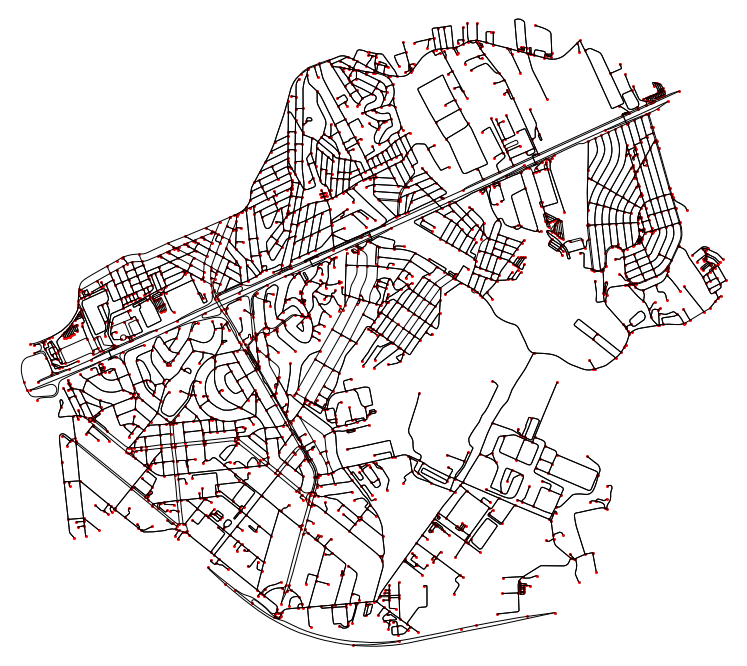
\includegraphics[width=.98\linewidth]{images/5_emp_bebidas/street_network_analysis/cumbica_malha_color.png}
        \label{fig:Cumbica_network_example}
    \end{subfigure}
    \begin{subfigure}{.46\textwidth}
        \centering
        % include second image
        \caption{conectividade dos nós}
        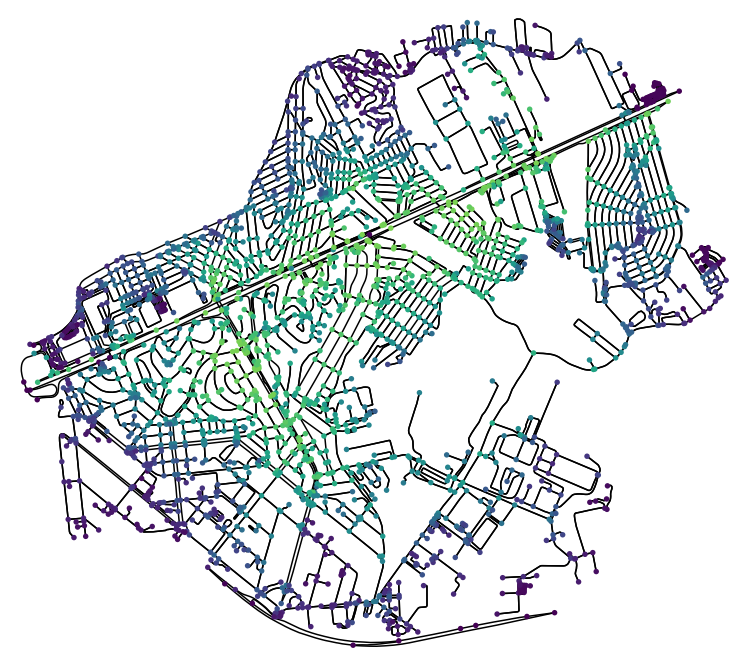
\includegraphics[width=.98\linewidth]{images/5_emp_bebidas/street_network_analysis/network_centrality_cumbica.png}
        \label{fig:network_centrality_cumbica}
    \end{subfigure}
    \caption*{\ Fonte: Produzido pelos autores Fernandes \& Alves}
 \end{figure}

\begin{figure}[htb]
    \centering
    \caption{Histograma de distribuição da orientação de vias de Cumbica - Guarulhos}
    \begin{subfigure}{.45\textwidth}
        \centering
        % include first image 
        \caption{Histograma em projeção linear}
        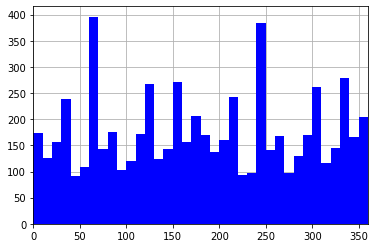
\includegraphics[height=0.6\textwidth]{images/5_emp_bebidas/street_network_analysis/histogram_cumbica.png}
        \label{fig:Cumbica_bearing_example_histogram}
    \end{subfigure}
    \begin{subfigure}{.45\textwidth}
      \centering
      % include second image
      \caption{Histograma em projeção polar}
      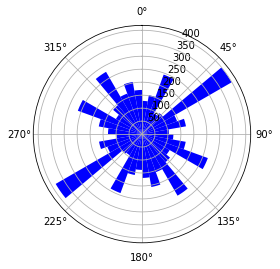
\includegraphics[height=0.6\textwidth]{images/5_emp_bebidas/street_network_analysis/polar_plot_cumbica.png}
      \label{fig:Cumbica_bearing_example_polarplot}
    \end{subfigure}
    \caption*{\ Fonte: Produzido pelos autores Fernandes \& Alves}
\end{figure}

%%%%%%%%%%%%%%%%%%%%%%%%%%%%%%%%%%%%%%%%%%%%%
\subsection{Resultado para os demais bairros}

Começando pelo problema de orientação, utiliza-se uma estrutura de laço do \textit{Python} para iterar sobre os diferentes bairros e realizar os cálculos de orientação um a um, entregando como resultado um histograma de projeção polar que pode ser utilizado posteriormente.
As Figuras \ref{fig:piorbairro_label} e \ref{fig:melhorbairro_label} apresentam exemplos de histogramas polares comparados com a estrutura da malha viária de dois bairros distintos, sendo eles o pior e o melhor cenário em termos de repasses.
Esta comparação permite associar a distribuição de orientações aos valores de repasses, porém curiosamente o bairro que apresentou um dos menores percentuais de repasse é caracterizado por um maior graus de ordenação do arranjo das vias, resultado este que vai na contra-mão da intuição e surpreendeu os autores num primeiro momento.

Por outro lado, a Figura \ref{fig:bearing_bairros} consolida todos histogramas polares em uma única imagem, permitindo uma visualização completa dos resultados.

E finalmente são geradas as estatísticas descritivas para cada um dos bairros, sendo os resultados completos apresentados na Tabela \ref{tab:resultados_completos} do capítulo de apêndice \ref{sec:appResultMalha}, valores estes que podem ser combinados a fim de se investigar existência de alguma correlação entre os valores gerados e os indicadores de repasse e devolução já introduzidos anteriormente. 

\begin{figure}[htb]
    \centering
    % Include first image
    \caption{Resultados para o bairro ``Lavras'', o que representa maior taxa de repasses (11.07\%) e índice de devolução acima da média (5.72\%)}
    \begin{subfigure}{0.42\textwidth}
        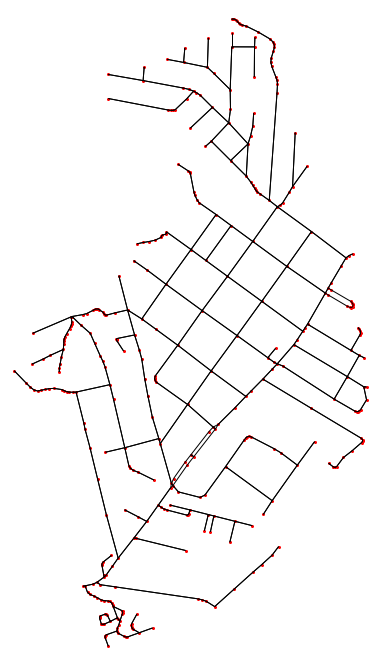
\includegraphics[height=0.75\textwidth]{images/5_emp_bebidas/street_network_analysis/Lavras_malha.png}
    \end{subfigure}
    % Include 2nd image
    \begin{subfigure}{0.42\textwidth}
        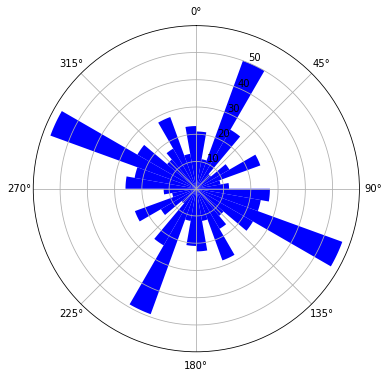
\includegraphics[height=0.75\textwidth]{images/5_emp_bebidas/street_network_analysis/Lavras_polar_plot.png}
    \end{subfigure}
    \caption*{\ Fonte: Produzido pelos autores Fernandes \& Alves}
    \label{fig:piorbairro_label}
\end{figure} % Pior bairro

\begin{figure}[htb]
    \centering
    % Include first image
    \caption{Resultados para o bairro ``Ponte Grande'', o qual apresenta um dos menores índices de repasse (2.44\%) e taxa de devolução abaixo da média (2.03\%)}
    \begin{subfigure}{0.42\textwidth}
        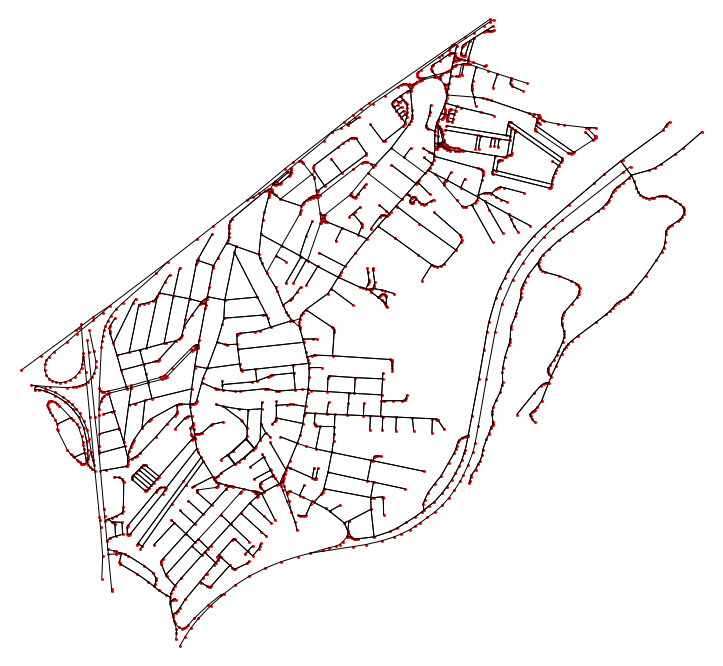
\includegraphics[height=0.75\textwidth]{images/5_emp_bebidas/street_network_analysis/Ponte_grande_malha.png}
    \end{subfigure}
    % Include 2nd image
    \begin{subfigure}{0.42\textwidth}
        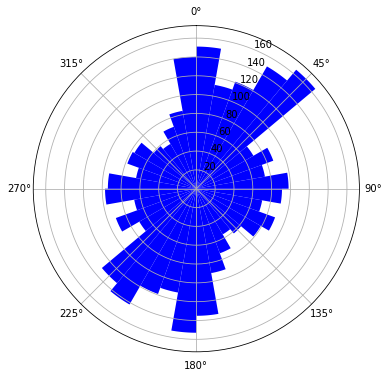
\includegraphics[height=0.75\textwidth]{images/5_emp_bebidas/street_network_analysis/ponte_grande_polar_plot.png}
    \end{subfigure}
    \caption*{\ Fonte: Produzido pelos autores Fernandes \& Alves}
    \label{fig:melhorbairro_label}
\end{figure} % Melhor bairro

%%%%%%%%%%%%%%%%%%%%%%%%%%%%%%%%%%%%%%%%%%%%%%%%%%%%%%%%%%%%%%%
\section{Relação entre as medidas estudadas} \label{sec:relMetricasBebidas}

Na presente seção, busca-se apresentar os resultados finais de corrrelação das variáveis-problema com os indicadores de malha e de fator de circuito apresentados nas seções anteriores. Assim, na Subseção \ref{FC_repBebidas}, é apresentada a análise de correlação do fator de circuito com o repasse. Já na Subseção \ref{ImpactoMalhaViariaBebidas}, é apresentada a análise dos resultados de correlação obtidos entre os indicadores da estrutura viária com os repasses e as devoluções.

%%%%%%%%%%%%%%%%%%%%%%%%%%%%%%%%%%%%%%%%%%%%%%%%%%%
\subsection{Fator de circuito e repasses} \label{FC_repBebidas}

A partir dos dados de fator de circuito calculados na Seção \ref{sec:AMBEV_FC}, é possível gerar um comparativo entre eles e os repasses. O objetivo da presente subseção é avaliar o efeito que o fator de circuito pode ter sobre a operação da empresa de bebidas brasileira a partir da perspectiva dos repasses.

Para a quantidade de repasses, os PDEs foram agrupados por bairros, ou seja, foi estudada a média do fator de circuito em relação ao total de repasses consolidado por bairros. 
%
Essa alternativa se mostrou eficaz para aliviar as discrepâncias entre os valores de repasse apresentados pelos mais de 4.000 PDEs.
%
A Figura \ref{fig:FC_repasse} apresenta a correlação obtida.
%
É possível observar no gráfico um certo grau de espalhamento dos pontos em suas relações de repasse e Fator de Circuito. 
Apesar da curva de tendência apresentada, identifica-se a presença de um ponto muito distante dos demais (\textit{outlier}), o que contribui significativamente para a tendência positiva da reta.

\begin{figure}[htb]
    \centering
    \caption{Correlação entre quantidade de repasses e fator de circuito médio por bairro}
    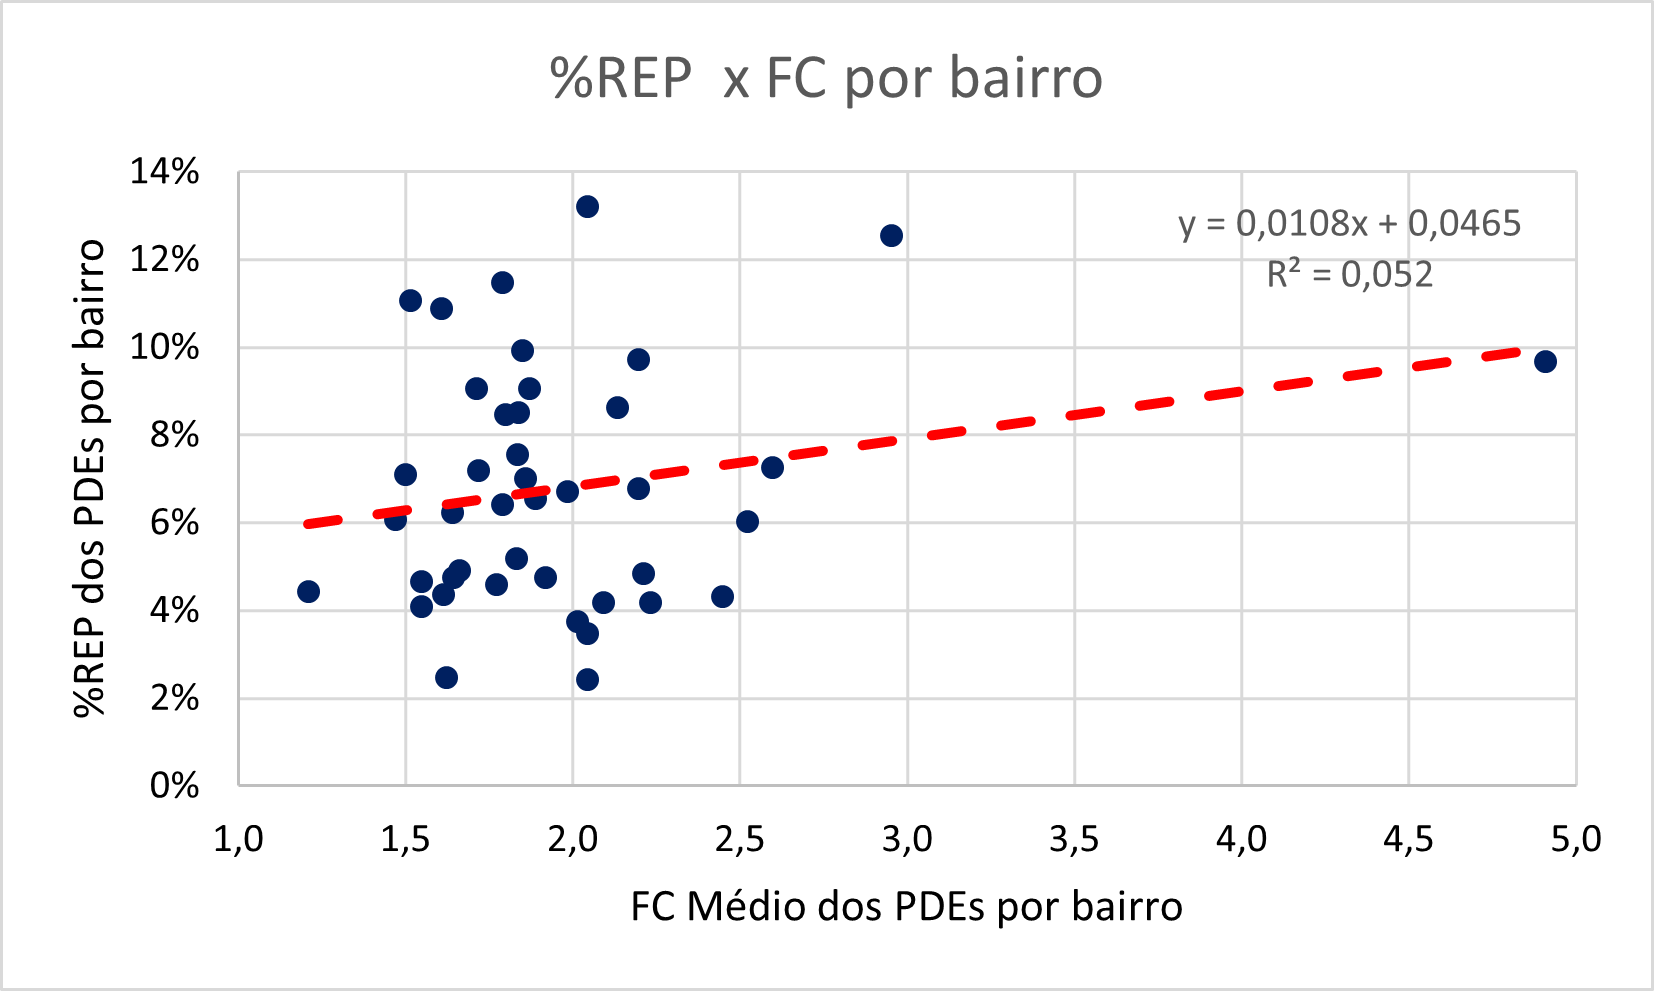
\includegraphics[width=0.8\textwidth]{images/5_emp_bebidas/excel_based/FC_bairros_novo.png}
    \caption*{\ Fonte: Produzido pelos autores Fernandes \& Alves}
    \label{fig:FC_repasse}
\end{figure}


%%%%%%%%%%%%%%%%%%%%%%%%%%%%%%%%%%%%
\subsection{Impacto da malha viária} \label{ImpactoMalhaViariaBebidas}

Em sequência, busca-se avaliar, para além do fator de circuito, como que os indicadores da estrutura viária obtidos na Seção \ref{sec:AMBEV_MalhaViaria} relacionam-se com os repasses e as devoluções do estudo de caso a partir do conceito de correlação linear simples, apresentado na Seção \ref{RegressoesLineares}.

Para tal, a Tabela \ref{tab:correlacao}, presente nos apêndices, apresenta os coeficientes de correlação de Pearson entre as principais variáveis obtidas no problema.
Nela, é possível extrair que as principais variáveis explicativas da quantidade de repasses por bairro são o comprimento total de vias naquele bairro e a quantidade de nós e de arcos, bem como a quantidade de intersecções.
Estas variáveis também explicam bem os valores de caixas devolvidas, que neste caso representa a devolução total por bairro.
Contudo nota-se que as correlações são mais fortes quando se analisam valores absolutos de devoluções e repasses por bairro em vez de valores relativos ou normalizados.

Nesse sentido, os resultados obtidos através da abordagem adotada sugerem que as principais variáveis explicativas do total de caixas devolvidas por bairro seriam o comprimento total de vias ($r=0,851$), número total de arcos ($r=0,787$), número total de nós ($r=0,770$) e quantidade total de intersecções ($r=0,767$), nesta ordem.
Todos estes valores positivos de coeficiente de regressão indicam uma tendência de haver maior quantidade de devoluções conforme se aumenta a complexidade da malha, representada pela quantidade total de seus elementos.
Já quanto à quantidade de repasses por bairros, obtém-se conclusões análogas.

Infelizmente o parâmetro $k\_average$, que representa a média de ângulos de incidência dos arcos sobre os nós, não apresentou nenhuma correlação consideravelmente alta em relação aos outros atributos estudados, o que pode ser de certa forma compreendido também pelos resultados apresentados nas Figuras \ref{fig:piorbairro_label} e \ref{fig:melhorbairro_label}. 
Havia uma expectativa de um comportamento correlato entre o indicador e as variáveis-problema estudadas devido ao estudo realizado para com os radares direcionais das vias de cada bairro. O parâmetro $k\_average$, porém, é uma representação bastante limitada dos radares direcionais, por retratar a média, somente, e não o comportamento de espalhamento dos mesmos.